%!TEX root=../Thesis_Zepeng.tex
\chapter{Numerical implementation and validation}\label{chp:6}
\minitoc
\section{Experimental verification}

\subsection{Introduction}
The aim of this chapter is to validate the predictive model proposed. This consists in simulating tests available in the literature to determine the lifetime at initiation of crack by the application of the model and to compare these with the experimental lifetimes. The validation of the model involves a wide variety of metallic materials. The loads tested are of two types: cyclic loading of multiaxial stress of constant amplitude and repeated sequences of uniaxial stresses of variable amplitudes. The fatigue data of the materials used and the loads tested are taken from laboratory experiments or the literature.

\newpage
\subsection{Random amplitude 1D tests from Cetim on AW-6106 T6 aluminum}

What makes automobile fatigue so difficult to predict is that, unlike standard tests done in a laboratory, an automobile's structure has to endure a complex, mostly random, set of static as well as cyclical stresses when in service, such as in \figref{complexloading} which could represent load data from testing or measurement, extracting the cyclic information can be challenging. 
\begin{figure}[h!]
	\centering
	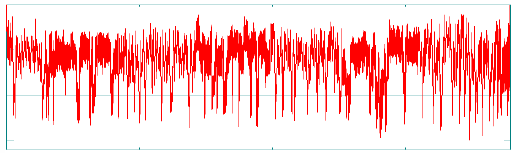
\includegraphics[width=\textwidth]{figures//complexloading.png} 
	\caption{Complex Cyclic Loading}
	\label{complexloading}
\end{figure}

As we mentioned before, the mean value of $\alpha$ depends on the loading pattern(sinusoidal, linear division points between max and min stresses in unit cycle,...), but the our optimal time step numerical strategy is not loading pattern dependent because it equally divides the range of $\alpha$ during the load history, which means it only concerns the variation amplitude of stress intensity. So in random loading case with only recorded maximum and minimum load history, we divide linearly between every 2 recorded points into $100$ time steps, and issue numerical results with optimal time step method.

The tests are performed on aluminum batches, the characteristics of the sample are shown in table.\ref{tab:cetim}.
\begin{figure}[!h]
\centering
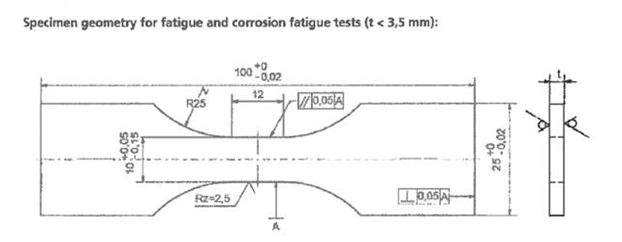
\includegraphics[width=0.7\textwidth]{figures//aluminum_cetim.png} 
\caption{Specimen geometry for fatigue tests of AW-6106 T6 aluminum}
\label{fig:aluminum}
\end{figure}
\begin{table}[!h]
\centering
\begin{tabular}{ll}
\hline
\textbf{Parameters}                                         & \textbf{Value}                    \\ \hline
Young's modulus                                             & $E=72$ GPa                       \\
Hardening parameter                                         &  $k=8.5$ MPa \\
Macroscopic yield stress                                    & $\sigma_y=230$ MPa              \\
Thickness & $e=2.9mm$                        \\
Width		 & $l= 9.95mm$                        \\ \hline
\end{tabular}
\caption{Material parameters}
\label{tab:cetim}
\end{table}

There are 12 validated uniaxial fatigue tests on the AW-6106 T6 aluminum sample, in which 2 are constant amplitude load case and 10 random  load case. 
The cyclic stress of test number 1(ep01) and test number 2(ep02) are respectively $131.9MPa$ and $97.0MPa$. We first identify the same parameters feasible to both loading cases. 

\begin{figure}[!h]
\centering
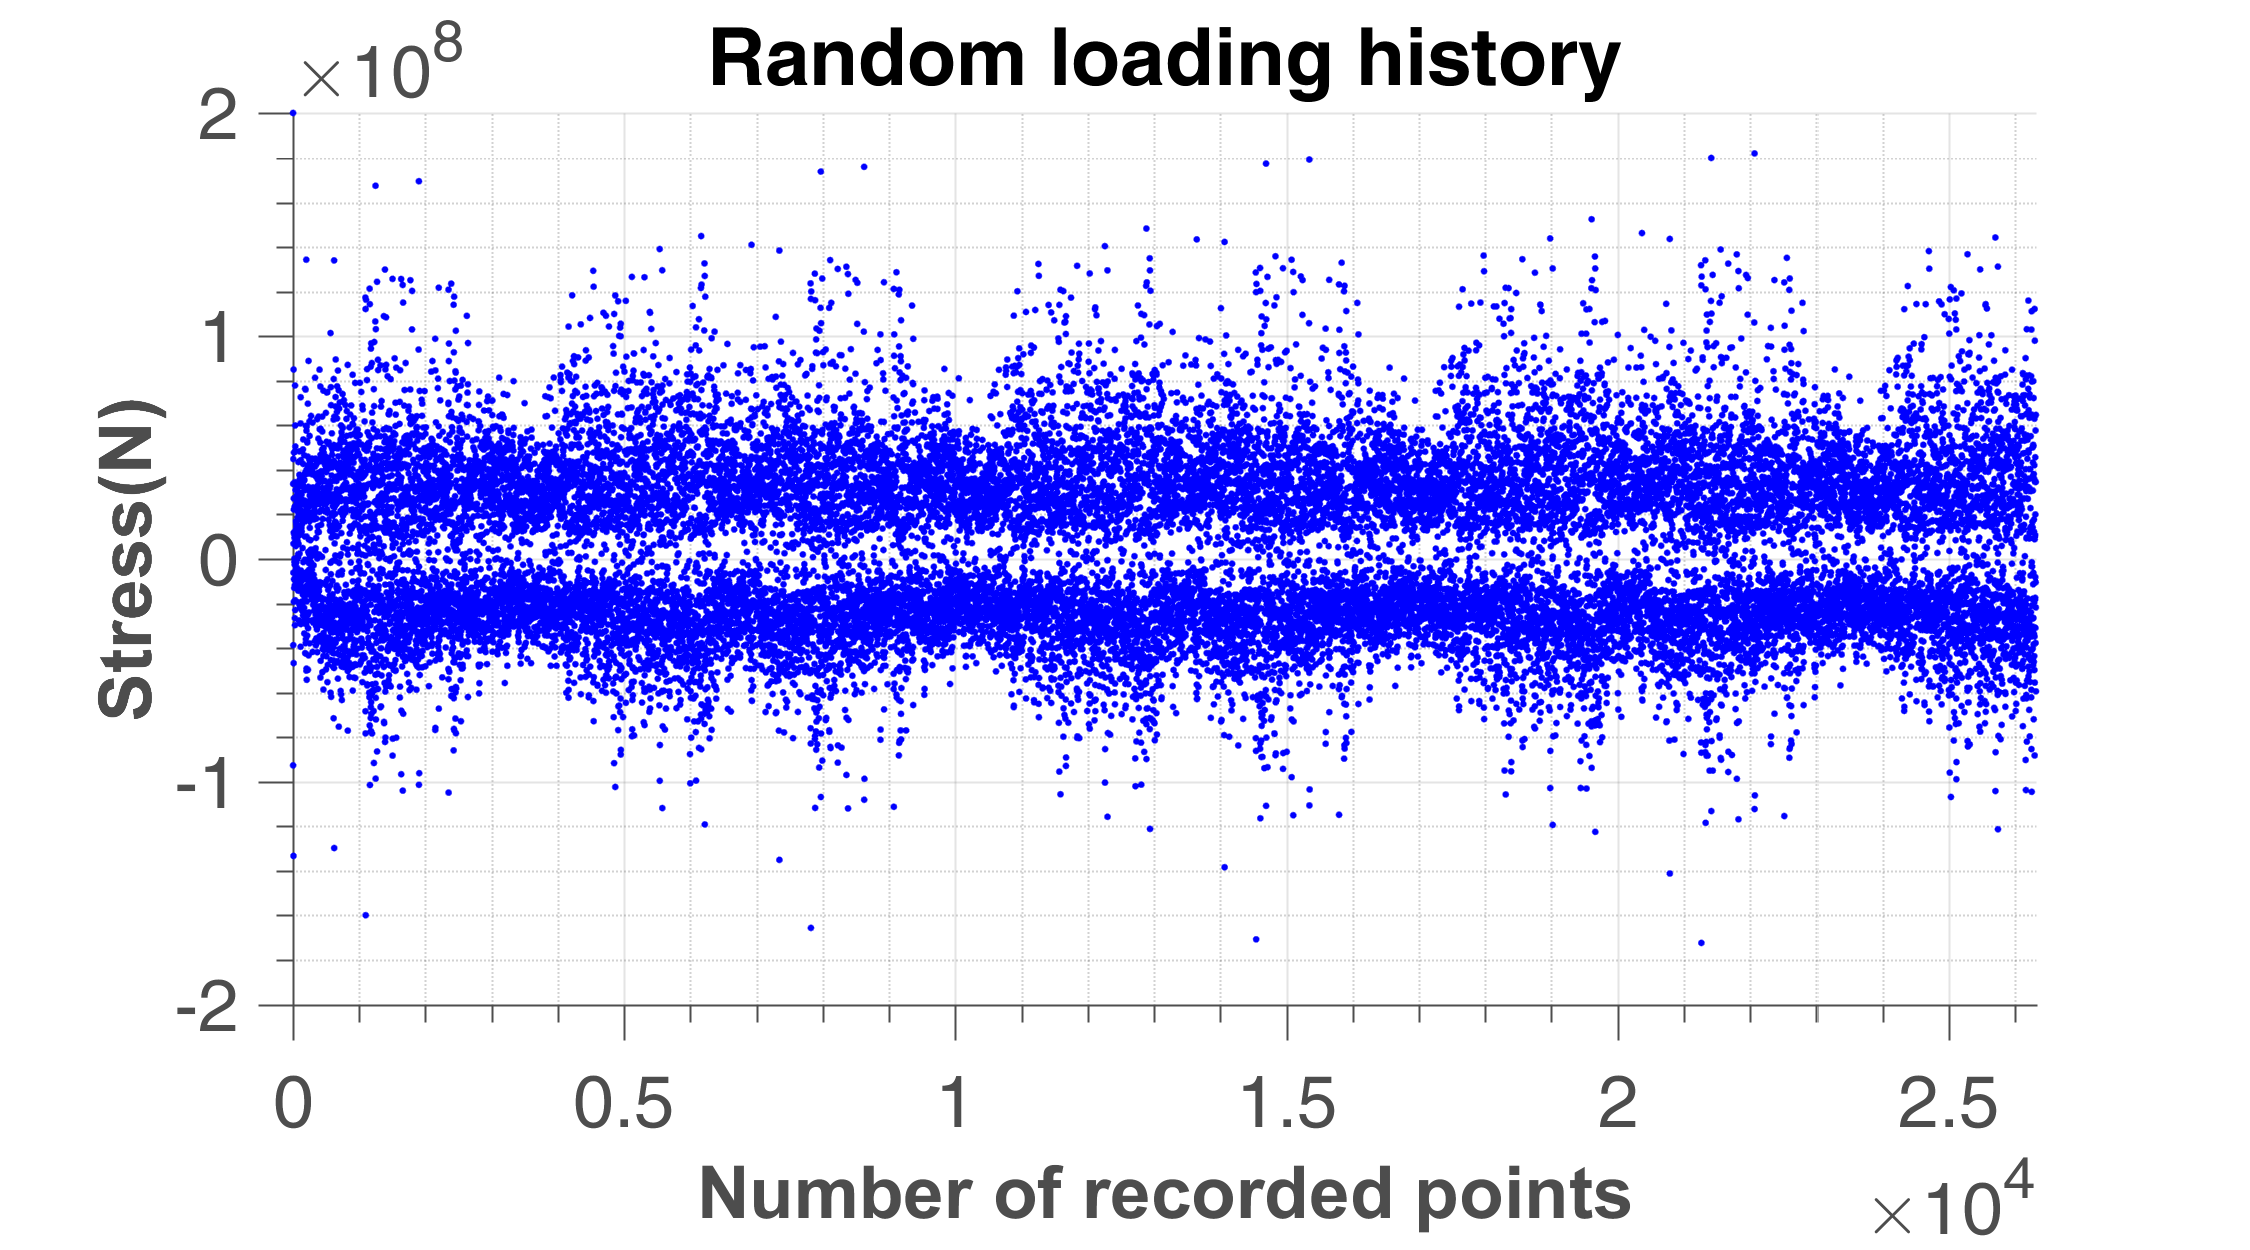
\includegraphics[width=\textwidth]{figures//EP_a_06_random.png} 
\caption{Random loading history on batch 06 of AW-6106 T6 aluminum}
\end{figure}	
The detailed tests information are shown in table.\ref{tab:Cetim}. There are 27000($\pm 2.4\%$) recorded points per repetition. 

\begin{table}[!h]
\centering
\begin{tabular}{lllll}
\hline
\textbf{Specimen} & \textbf{Fmax (kN)} & \textbf{$\Sigma_{max}$ in the block} & \textbf{Number of repetition} & \textbf{Number of points} \\ \hline
BATCH\_A\_01      & 3.375              &                                      &                                          & 99892                                \\
BATCH\_A\_02      & 2.475              &                                      &                                          & 414298                               \\
BATCH\_A\_04      & nom                & 225.88                               & 95                                       & 2500000                              \\
BATCH\_A\_05      & nom                & 225.88                               & 156                                      & 4105263                              \\
BATCH\_A\_06      & nom                & 225.88                               & 145                                      & 3815789                              \\
BATCH\_A\_07      & nom                & 225.88                               & 90                                       & 2368421                              \\
BATCH\_A\_08      & nom                & 225.88                               & 194                                      & 5105263                              \\
BATCH\_A\_09      & nom                & 225.88                               & 197                                      & 5184211                              \\
BATCH\_A\_10      & nom x 0,9          & 203.292                              & 515                                      & 13552632                             \\
BATCH\_A\_11      & nom x 0,9          & 203.292                              & 385                                      & 10131579                             \\
BATCH\_A\_12      & nom x 0,9          & 203.292                              & 424                                      & 11157895                             \\
BATCH\_A\_13      & nom x 0,9          & 203.292                              & 409                                      & 10763158                             \\ \hline
BATCH\_B\_01      & nom                & 225.88                               & 121                                      & 3184211                              \\
BATCH\_B\_02      & nom x 0,8          & 180.704                              & 380                                      & 10000000                             \\
BATCH\_B\_03      & nom x 0,8          & 180.704                              & 380                                      & 10000000                             \\
BATCH\_B\_04      & nom x 0,9          & 203.292                              & 406                                      & 10684211                             \\
BATCH\_B\_05      & nom x 0,9          & 203.292                              & 454                                      & 11947368                             \\
BATCH\_B\_06      & nom x 0,9          & 203.292                              & 518                                      & 13631579                             \\
BATCH\_B\_07      & nom x 0,9          & 203.292                              & 553                                      & 14552632                             \\
BATCH\_B\_08      & nom x 0,9          & 203.292                              & 612                                      & 16105263                             \\
BATCH\_B\_09      & nom                & 225.88                               & 253                                      & 6657895                              \\
BATCH\_B\_10      & nom                & 225.88                               & 196                                      & 5157895                              \\
BATCH\_B\_11      & nom                & 225.88                               & 178                                      & 4684211                              \\
BATCH\_B\_12      & nom                & 225.88                               & 123                                      & 3236842                              \\ \hline
\end{tabular}
\caption{Cetim fatigue tests result on AW-6106 T6 aluminum}
\label{tab:Cetim}
\end{table}

We assume the material parameters like Young's modulus, hardening parameter, hydrostatic pressure sensitivity, macroscopic yield stress, Wohler curve exponent and sequence effect parameters are known. We first identify the weakening scales distribution, and dissipated energy to failure from cyclic tests ep01 and ep02. Then change the parameter $n_0$ to see if our assumption is correct or need to be changed. 


The numerical fitting process show that the damage is caused mainly by large stresses. The definition of major stress now need to be specified according to the material. To take into account this effect we first find out the proportion stress above a certain value in the repetition signal of random loading, as shown in Table.\ref{tab.majordamage}.  Here ep\_a and ep\_b are the same material. Since the samples were extracted from aluminum profiles of industrial products,  the two batches correspond to two different times of sampling in the production. The variation is supposed to be representative of the regular tolerances you might have in the production. ep\_a\_01 and ep\_a\_02 are constant amplitude loading which helps identify the power of weakening scale distribution $\beta$. ep\_a\_03 is low cycle fatigue data.  ep\_b\_02 and ep\_b\_03 have infinite life time. The data in the table are grabbed from random signal high cycle fatigue loading history.

\begin{table}[!h]
\centering
\begin{tabular}{llllllll}
\hline
\textbf{Stress(MPa)\textgreater}  & \textbf{70}    & \textbf{90}    & \textbf{110}   & \textbf{130}    & \textbf{150}    & \textbf{170}    & \textbf{190}    \\
\textbf{$S_{a}$(MPa)\textgreater} & \textbf{57.15} & \textbf{73.48} & \textbf{89.81} & \textbf{106.14} & \textbf{122.47} & \textbf{138.80} & \textbf{155.13} \\ \hline
\textbf{ep\_a\_04}           &                & 1.962\%        & 0.904\%        & 0.077\%         & 0.037\%         & 0.018\%         & 0.007\%         \\
\textbf{ep\_a\_05}           &                & 1.604\%        & 0.784\%        & 0.044\%         & 0.030\%         & 0.007\%         & 0.007\%         \\
\textbf{ep\_a\_06}           &                & 1.645\%        & 0.784\%        & 0.045\%         & 0.030\%         & 0.007\%         & 0.007\%         \\
\textbf{ep\_a\_07}           &                & 1.632\%        & 0.788\%        & 0.048\%         & 0.029\%         & 0.007\%         & 0.007\%         \\
\textbf{ep\_a\_08}           &                & 1.644\%        & 0.787\%        & 0.048\%         & 0.037\%         & 0.007\%         & 0.007\%         \\
\textbf{ep\_a\_09}           &                & 1.655\%        & 0.800\%        & 0.048\%         & 0.037\%         & 0.007\%         & 0.007\%         \\
\textbf{ep\_a\_10}           &                & 0.768\%        & 0.134\%        & 0.007\%         & 0.000\%         & 0.000\%         & 0.000\%         \\
\textbf{ep\_a\_11}           &                & 0.772\%        & 0.145\%        & 0.007\%         & 0.000\%         & 0.000\%         & 0.000\%         \\
\textbf{ep\_a\_12}           &                & 0.779\%        & 0.133\%        & 0.011\%         & 0.000\%         & 0.000\%         & 0.000\%         \\
\textbf{ep\_a\_13}           &                & 0.775\%        & 0.141\%        & 0.007\%         & 0.000\%         & 0.000\%         & 0.000\%         \\ \hline
\textbf{ep\_b\_01}           & 4.739\%        & 1.737\%        & 0.840\%        & 0.224\%         & 0.049\%         & 0.034\%         & 0.004\%         \\
\textbf{ep\_b\_04}           & 1.999\%        & 0.745\%        & 0.156\%        & 0.034\%         & 0.004\%         & 0.000\%         & 0.000\%         \\
\textbf{ep\_b\_05}           & 2.010\%        & 0.749\%        & 0.148\%        & 0.034\%         & 0.008\%         & 0.000\%         & 0.000\%         \\
\textbf{ep\_b\_06}           & 1.999\%        & 0.790\%        & 0.118\%        & 0.034\%         & 0.008\%         & 0.000\%         & 0.000\%         \\
\textbf{ep\_b\_07}           & 2.029\%        & 0.756\%        & 0.152\%        & 0.034\%         & 0.008\%         & 0.000\%         & 0.000\%         \\
\textbf{ep\_b\_08}           & 1.999\%        & 0.737\%        & 0.137\%        & 0.034\%         & 0.008\%         & 0.000\%         & 0.000\%         \\
\textbf{ep\_b\_09}           & 4.663\%        & 1.687\%        & 0.798\%        & 0.205\%         & 0.049\%         & 0.034\%         & 0.004\%         \\
\textbf{ep\_b\_10}           & 4.712\%        & 1.744\%        & 0.809\%        & 0.224\%         & 0.046\%         & 0.034\%         & 0.004\%         \\
\textbf{ep\_b\_11}           & 4.636\%        & 1.664\%        & 0.790\%        & 0.209\%         & 0.049\%         & 0.034\%         & 0.004\%         \\
\textbf{ep\_b\_12}           & 0.775\%        & 0.141\%        & 0.007\%        & 0.000\%         & 0.000\%         & 0.000\%         & 0.000\%         \\ \hline
\end{tabular}
\caption{Proportion of stress(MPa) above which there is major damage with $\Sigma_y$=230MPa, test data provided by CETIM on AW-6106 T6 aluminum.}
\label{tab.majordamage}
\end{table}

\begin{table}[!h]
\centering
\begin{tabular}{lrrrrrrr}
\hline
\multicolumn{8}{c}{\textbf{Random amplitude sensitivity test with $f(\beta)=\beta$}}                                                                                                                                                                                                                                             \\ \hline
& \multicolumn{1}{r}{\textbf{Ref}} & \multicolumn{1}{r}{\textbf{Min}} & \multicolumn{1}{r}{\textbf{Max}} & \multicolumn{1}{r}{\textbf{Ref\_n}} & \multicolumn{1}{r}{\textbf{Min\_n}} & \multicolumn{1}{r}{\textbf{Max\_n}} & \multicolumn{1}{r}{\textbf{Sensitivity}} \\ \hline
\textbf{$\beta$}   & 1.1                                          & 1.05                             & 1.50                             & 4220452                                    & 7469257                             & 1799585                             & -3.28 
\\
\textbf{$\lambda$} & 0.1                                          & 0.05                             & 0.50                             & 4220452                                   & 4566335                             & 2175991                             & -0.13                                    \\
\textbf{$W_0$}     & 3.27e8                                     & 1.00e8                         & 5.00e8                         & 4220452                                    & 1321761                             & 6420810                             & 0.99                                    \\
\textbf{$a$}       & 0.1                                          & 0.05                             & 0.15                             & 4220452                                   & 7156622                             & 2827894                             & -1.03                                   \\ \hline
\end{tabular}
\caption{Parameters sensitivity at random loading of ep05 on AW-6106 T6 aluminum}
\label{tab.sensitivity_random1}
\end{table}

From Table.\ref{tab.sensitivity_const2} and Table.\ref{tab.sensitivity_random2} we can see $f(\beta)$ has positive correlation with $\beta$ in high cycle fatigue which is the regime we focus on. So we give $f(\beta)=\beta$ in high cycle random loading case to minimize the parameters to collaborate.
\begin{table}[!h]
\centering
\begin{tabular}{lrrrrrrr}
\hline
\multicolumn{8}{c}{\textbf{Constant amplitude sensitivity test with $f(\beta)\neq\beta$}}                                                                                                                                                                                                 \\ \hline
& \multicolumn{1}{l}{\textbf{Ref}} & \multicolumn{1}{l}{\textbf{Min}} & \multicolumn{1}{l}{\textbf{Max}} & \multicolumn{1}{l}{\textbf{Ref\_n}} & \multicolumn{1}{l}{\textbf{Min\_n}} & \multicolumn{1}{l}{\textbf{Max\_n}} & \multicolumn{1}{l}{\textbf{Sensitivity}} \\ \hline
\textbf{$\beta$}    & 1.1                              & 1.05                             & 1.50                             & 414233                              & 797377                              & 213682                              & -3.44                                    \\
\textbf{$\lambda$}  & 0.1                              & 0.05                             & 0.50                             & 414233                              & 449598                              & 443376                              & 0.00                                     \\
\textbf{$W_0$}      & 3.27e8                         & 1.00e8                         & 5.00e8                         & 414233                              & 137498                              & 687209                              & 1.08                                     \\
\textbf{$a$}        & 0.1                              & 0.05                             & 0.15                             & 414233                              & 672869                              & 324754                              & -0.84                                    \\
\textbf{$f(\beta)$} & 1.1                              & 1.05                             & 1.5                              & 414233                              & 441661          &511644          & 0.41                                     \\ \hline
\end{tabular}
\caption{Parameters sensitivity at cyclic loading of ep02 on AW-6106 T6 aluminum}
\label{tab.sensitivity_const2}
\end{table}
\begin{table}[!h]
\centering
\begin{tabular}{lrrrrrrr}
\hline
\multicolumn{8}{c}{\textbf{Random amplitude sensitivity test with $f(\beta)\neq\beta$}}                                                                                                                                                                                                   \\ \hline
\textbf{}           & \multicolumn{1}{l}{\textbf{Ref}} & \multicolumn{1}{l}{\textbf{Min}} & \multicolumn{1}{l}{\textbf{Max}} & \multicolumn{1}{l}{\textbf{Ref\_n}} & \multicolumn{1}{l}{\textbf{Min\_n}} & \multicolumn{1}{l}{\textbf{Max\_n}} & \multicolumn{1}{l}{\textbf{Sensitivity}} \\ \hline
\textbf{$\beta$}    & 1.1                              & 1.05                             & 1.50                             & 4220452                             & 7254554                             & 2472791                             & -2.77                                    \\
\textbf{$\lambda$}  & 0.1                              & 0.05                             & 0.50                             & 4220452                             & 4566335                             & 2175991                             & -0.13                                    \\
\textbf{$W_0$}      & 3.27e8                         & 1.00e8                         & 5.00e8                         & 4220452                             & 1321761                             & 6420810                             & 0.99                                     \\
\textbf{$a$}        & 0.1                              & 0.05                             & 0.15                             & 4220452                             & 7156622                             & 2827894                             & -1.03                                    \\
\textbf{$f(\beta)$} & 1.1                              & 1.05                             & 1.5                              & 4220452                             & 4341560                             & 3052299                             & -0.75                                    \\ \hline
\end{tabular}
\caption{Parameters sensitivity at random loading of ep05 on AW-6106 T6 aluminum}
\label{tab.sensitivity_random2}
\end{table}
The sensitivity of parameters is calculated by dividing the percentage of variation of  number of points to failure with respect to the reference number of points to failure, by the percentage of variation of parameter with respect to the reference parameter. As is shown in Eq.\eqref{eq.sensitivity}.
\begin{equation}
sensitivity = \dfrac{\left( Max_n-Min_n\right)/Ref_n}{\left( Max-Min\right)/Ref}.
\label{eq.sensitivity}
\end{equation}



%The standard S-N curve is fitted with fatigue data provided by Cetim(the red line). Analytical calculation of mean dissipated energy and of the average value of $\alpha$ on one cycle, and  integration of the differential equation in D with these mean values is provided. The comparison with numerical method where we have changing $\alpha$ and $W$ at each time step in standard $S-N$ curve is shown in \figref{fig.para}:a. This analytical strategy is proposed to give a much cheaper way to treat cyclic loadings for high cycle fatigue. However, we find that there is a constant relative error between the analytical result and numerical one and the analytical one is more conservative. The relative error is due to integration of damage $D$ from Eq.\eqref{eq.DWcyc} to Eq.\eqref{eq.NFWcyc}. We assumed $\alpha$ is constant during damage accumulation which in step by step method is not the case.

%The influence of all the parameters on constant amplitude cyclic load using Eq.\eqref{eq.nf}  are shown in \figref{fig.para}.
%\begin{Figure}[!h]{The influence of parameters on the shape and limit of S-N curve}[fig.para]
%	\graphfile*[42]{figures//SNnumerical.png}[S-N curve using numerical and analytical method]
%	\graphfile*[42]{figures//SNlam.png}[The $\lambda$ influence on S-N curve]
%	\\
%    \graphfile*[42]{figures//SNa.png}[The $a$ influence on S-N curve]
%	\graphfile*[42]{figures//SNWF.png}[The $W_F$ influence on S-N curve]
%	\\
%	\graphfile*[42]{figures//SNb.png}[The $\beta$ influence on S-N curve]
%	\graphfile*[42]{figures//SNpb.png}[The $f(\beta)$ influence on S-N curve]
%\end{Figure}
%The different parameters impacts are shown in purple curves. We can see the weakening scale $\beta$ changes the inclination of S-N curve. $\beta$ is also the magnification factor which magnify large stress damage as well as minify small stress damage.  Not surprisingly the hydrostatic stress sensitivity $\lambda$ has more influence on large stress. The amplification factor of load intensity in damage accumulation $a$ and  energy scaling in damage accumulation law $W_0$ adapts to fatigue life without changing the shape the S-N curve.

The reference parameters value we use are in Tab.\ref{tab.cetim.alp}.  
\begin{table}[!h]
\centering
\begin{tabular}{lrrrr}
\hline
\textbf{Constant $\alpha$} & \textbf{$W_0$(MPa)} & \textbf{$\lambda$} & \textbf{$\beta$}  & \textbf{$\alpha$}\\
& 326.9         & 0.1               & 1.1            & 0.7                         \\ \hline
\textbf{Changing $\alpha$} & \textbf{$W_0$(MPa)} & \textbf{$\lambda$} & \textbf{$\beta$}  & \textbf{$a$}\\
& 326.9         & 0.1               & 1.1            & 0.1                         \\ \hline
\end{tabular}
\caption{The parameters in 1D cyclic and random loading on AW-6106 T6
aluminum fatigue tests by Cetim}
\label{tab.cetim.alp}
\end{table}

The best fitted results with constant $\alpha$ are shown in \figref{fig.Cetimerralpfix}. The dispersion is relatively large. In conclusion, we are not able to predict the random stress amplitude fatigue life with fixed $\alpha$, because random stresses not only cause different energy dissipations, but also have influence on damage accumulation speed, so we have to update the value of $\alpha$ at each time step. 

\begin{figure}[!h]
\centering
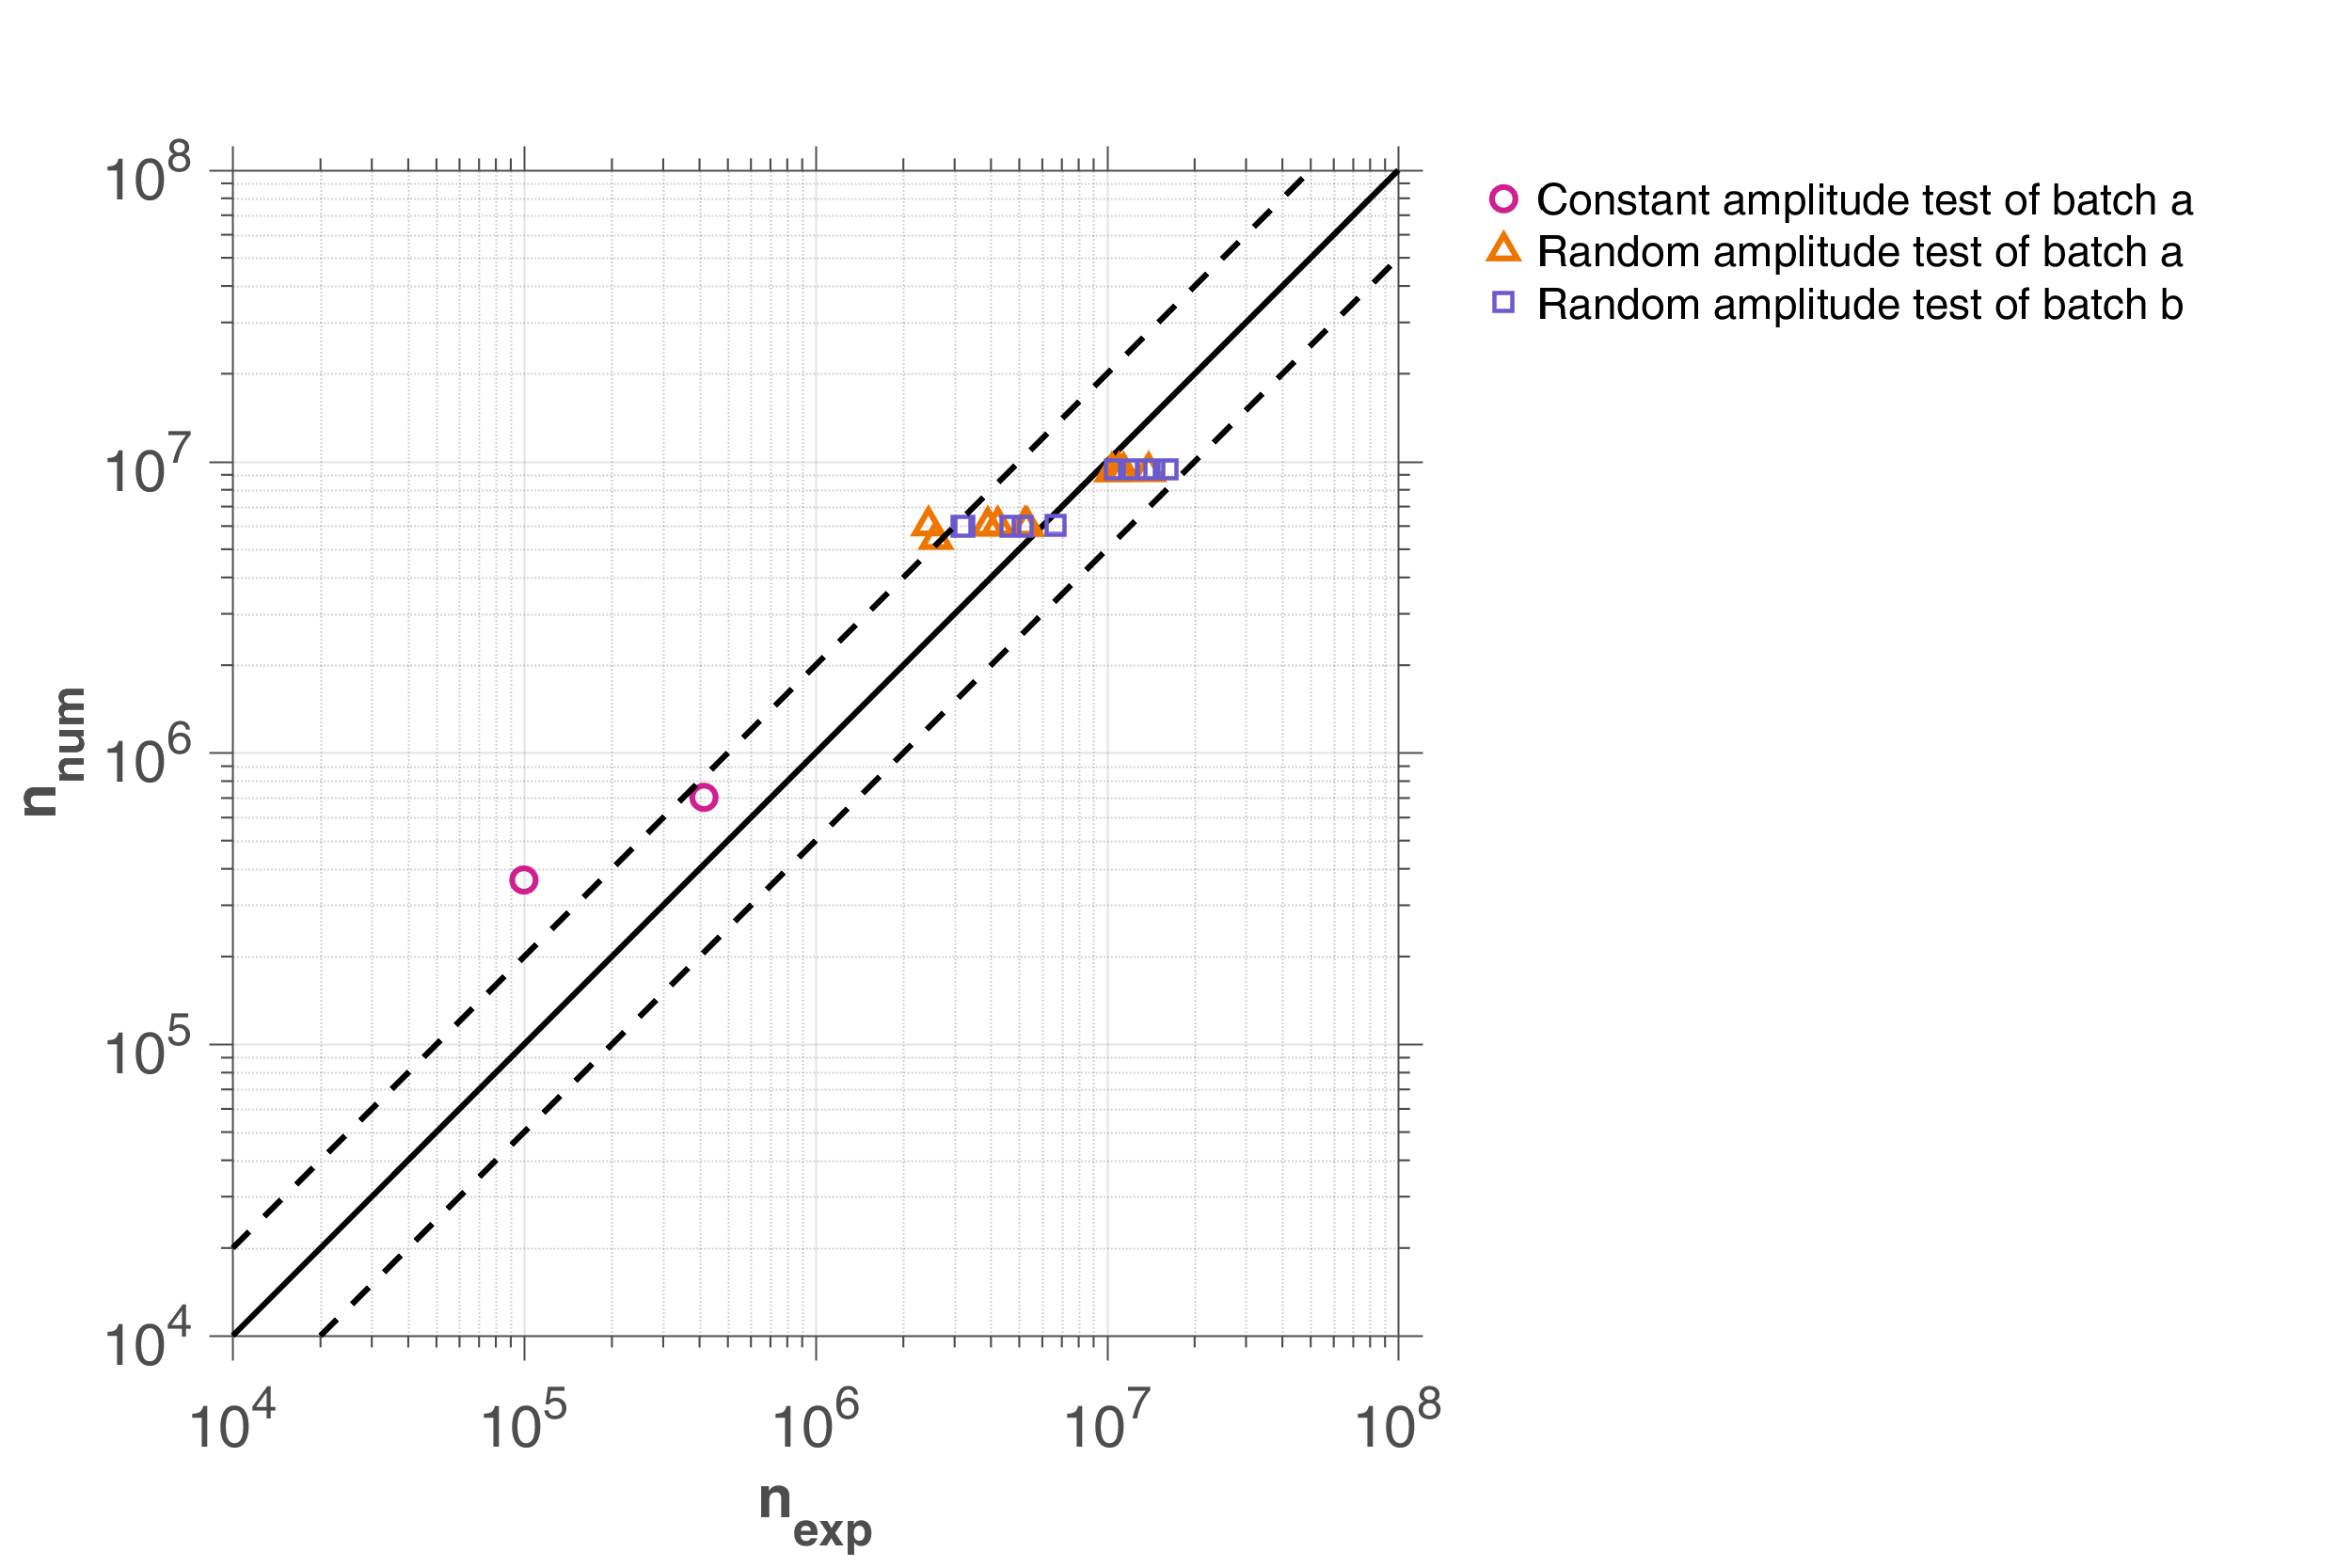
\includegraphics[width=\textwidth]{figures//Cetim_err_alpfix.png} 
\caption{Comparison between experimental and numerical results of 1D cyclic and random loading on aluminum fatigue tests by CETIM with constant $\alpha$}
\label{fig.Cetimerralpfix}
\end{figure}

We can find that the numerical results are satisfactory with major damage effect. The dispersion figure with distinction of major damage is depicted in \figref{fig.Cetimerr}. Here it is necessary to control the parameter $a$ to make sure $\alpha>0$ in the most severe situation.

\begin{figure}[!h]
\centering
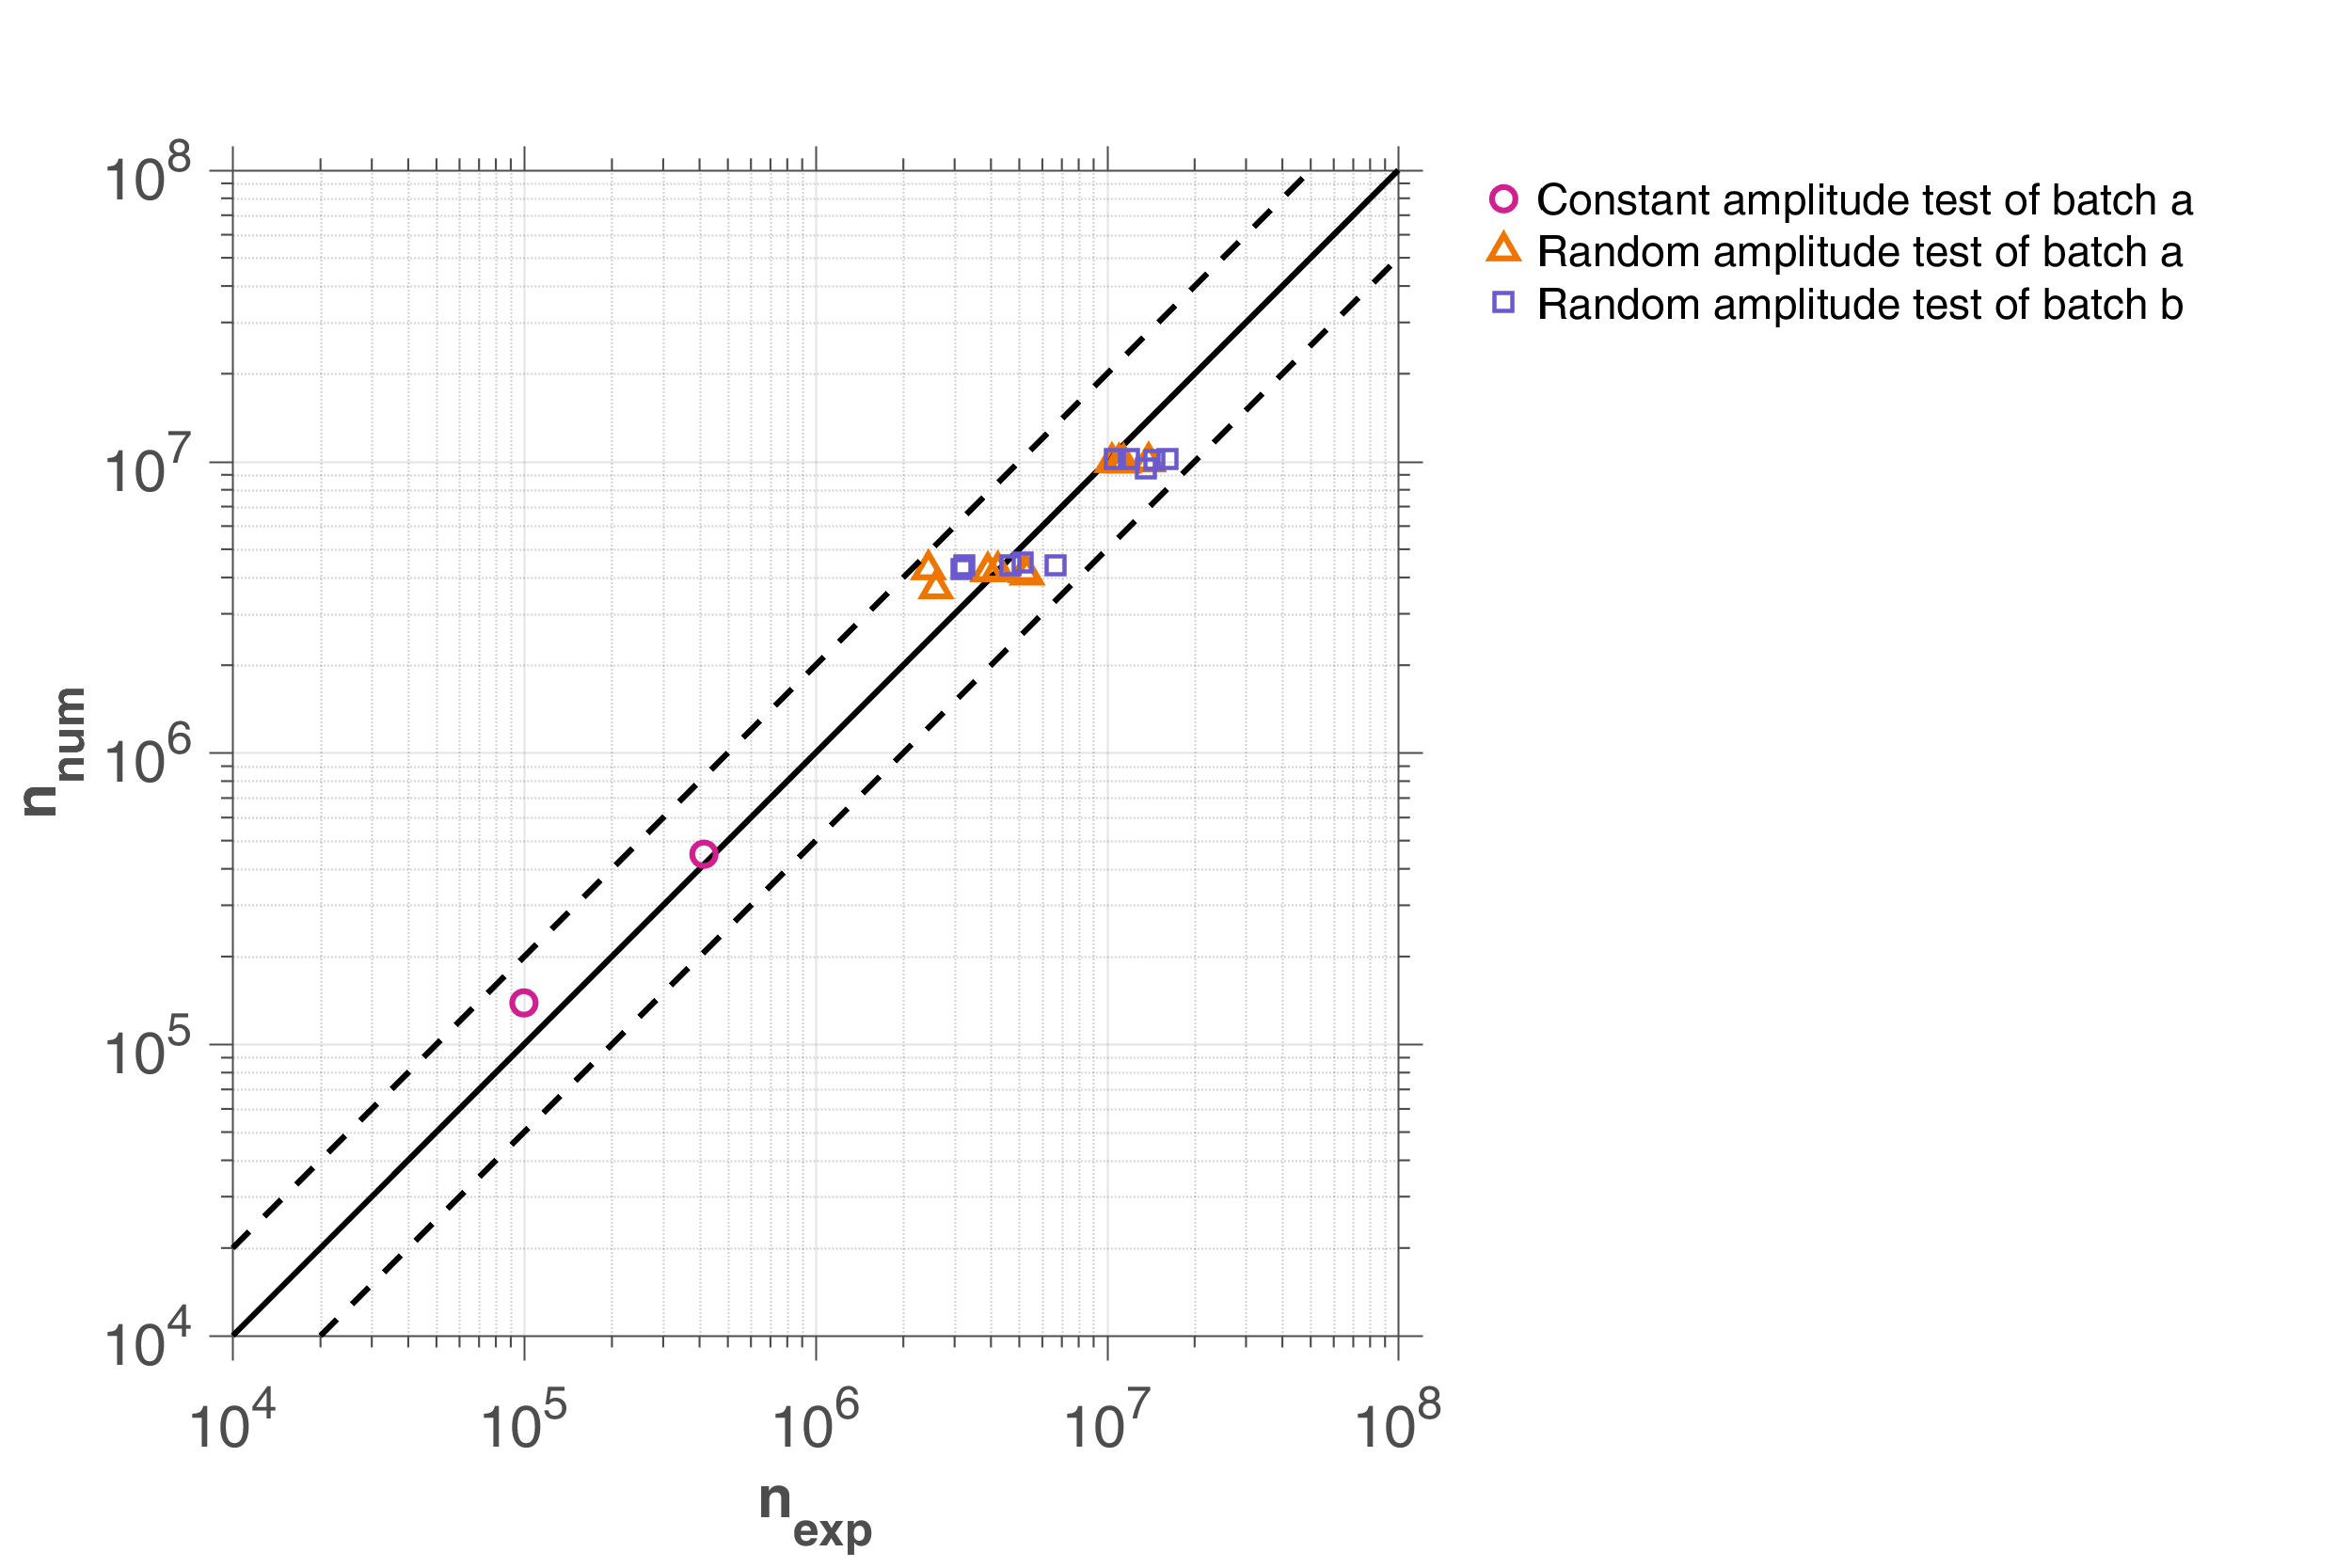
\includegraphics[width=\textwidth]{figures//Cetim_err.png} 
\caption{Comparison between experimental and numerical results of 1D cyclic and random loading on aluminum fatigue tests by Cetim}
\label{fig.Cetimerr}
\end{figure}

\clearpage
\subsection{Experimental validation of the model on aluminum 6082 T6}
\subsubsection{Presentation of aluminum 6082 T6}

The material tested is aluminum 6082 T6, used by \cite{susmel2003multiaxial} to validate their method of lifetime prediction. The mechanical properties of this material are summarized in Table.\ref{tab.al6082t6}.

\begin{table}[!h]
\centering
\begin{tabular}{|c|c|c|c|}
\hline
\textbf{$E${[}GPa{]}} & \textbf{$\sigma_{y}${[}MPa{]}} & \textbf{$\sigma_u${[}MPa{]}} & \textbf{$\nu$} \\ \hline
69.4                                  & 298                                & 343                         & 0.33                 \\ \hline
\end{tabular}
\caption{Mechanical and dynamic characteristics of aluminum 6082 T6 (\cite{susmel2003multiaxial})}
\label{tab.al6082t6}
\end{table}
\subsubsection{Specimens of aluminum 6082 T6}
The specimens were made from the drawn bars (diameter 30 mm) and the geometrical shape of which is given in \figref{fig:aluminum6082T6}. They are successively polished with 6-μm diamond compounds until a good mirror-like finish is obtained.
\begin{figure}[!h]
\centering
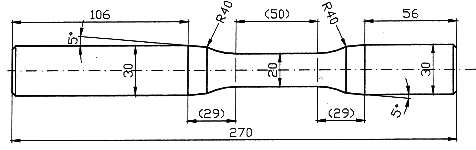
\includegraphics[width=0.7\textwidth]{figures//aluminum6082T6sample.png} 
\caption{Specimen geometry for fatigue tests of aluminum 6082 T6}
\label{fig:aluminum6082T6}
\end{figure}

\subsubsection{Fatigue tests on aluminum 6082 T6}
The simulated tests are purely alternate and summarized in Tables \ref{tab.AL6082T6BT1D} and \ref{tab.AL6082T6BT2D}. They consist of simple tests in bending, torsion and bending-torsion in phase and out-phase for two cases of biaxial stress ratio, $\lambda=\tau_{xy,a}/\sigma_{x,a}$
($\lambda>1$ and $\lambda<1$). The expected lifetimes range from $10^4$ to $1.5\times10^6$ cycles. 
\begin{table}[]
\centering
\begin{tabular}{|l|l|l|l|l|l|}
\hline
Batch $N^\circ$ & $\sigma_{x,a}${[}MPa{]} & $\tau_{xy,a}${[}MPa{]} & $\lambda$ & $\delta [^\circ]$ & $N_{f,5\%}${[}Cycles{]} \\ \hline
P1B1 & 190 & 0 & 0 & 0 & 160000 \\ \hline
P2B2 & 180 & 0 & 0 & 0 & 248518 \\ \hline
P3B3 & 164 & 0 & 0 & 0 & 444411 \\ \hline
P4B4 & 144 & 0 & 0 & 0 & 1069220 \\ \hline
P5B5 & 224 & 0 & 0 & 0 & 56285 \\ \hline
P6B4 & 145 & 0 & 0 & 0 & 1238325 \\ \hline
P7B1 & 187 & 0 & 0 & 0 & 200480 \\ \hline
P8B3 & 161 & 0 & 0 & 0 & 423590 \\ \hline
PC9T1 & 0 & 117 & $\infty$ & 0 & 534032 \\ \hline
PC10T2 & 0 & 155 & $\infty$ & 0 & 26987 \\ \hline
PC11T3 & 0 & 127 & $\infty$ & 0 & 76665 \\ \hline
PC12T3 & 0 & 127 & $\infty$ & 0 & 132295 \\ \hline
PC13T1 & 0 & 117 & $\infty$ & 0 & 203535 \\ \hline
PC14T2 & 0 & 155 & $\infty$ & 0 & 16195 \\ \hline
PC15T4 & 0 & 106 & $\infty$ & 0 & \textgreater1.1E6 \\ \hline
PC16T4 & 0 & 104 & $\infty$ & 0 & 565150 \\ \hline
\end{tabular}
\caption{Simple bending and torsion tests (R = -1)\cite{susmel2003multiaxial}}
\label{tab.AL6082T6BT1D}
\end{table}
\begin{table}[]
\centering
\begin{tabular}{|l|l|l|l|l|l|}
\hline
Batch $N^\circ$ & $\sigma_{x,a}${[}MPa{]} & $\tau_{xy,a}${[}MPa{]} & $\lambda$ & $\delta [^\circ]$ & $N_{f,5\%}${[}Cycles{]} \\ \hline
P17BT1 & 57 & 100 & 1.75 & 0 & 266435 \\ \hline
P18BT2 & 51 & 84 & 1.65 & 0 & 1119254 \\ \hline
P19BT2 & 51 & 84 & 1.65 & 0 & 1416225 \\ \hline
P20BT3 & 71 & 118 & 1.66 & 0 & 83000 \\ \hline
P21BT3 & 70 & 118 & 1.69 & 0 & 75695 \\ \hline
P22BT1 & 59 & 99 & 1.68 & 0 & 630325 \\ \hline
P23BT4 & 132 & 97 & 0.73 & 0 & 157210 \\ \hline
P24BT4 & 132 & 99 & 0.75 & 0 & 126470 \\ \hline
P25BT5 & 144 & 107 & 0.74 & 0 & 35450 \\ \hline
P26BT5 & 149 & 105 & 0.7 & 0 & 68465 \\ \hline
P27BT6 & 122 & 90 & 0.74 & 0 & 252658 \\ \hline
P28BT7 & 116 & 83 & 0.72 & 0 & 316149 \\ \hline
P30BT8 & 148 & 66 & 0.45 & 90 & 278836 \\ \hline
P31BT9 & 152 & 47 & 0.31 & 90 & 465010 \\ \hline
P32BT8 & 149 & 68 & 0.46 & 90 & 118965 \\ \hline
P33BT9 & 155 & 72 & 0.46 & 90 & 447525 \\ \hline
P34BT10 & 190 & 105 & 0.55 & 90 & 47940 \\ \hline
P35BT10 & 189 & 106 & 0.56 & 90 & 30995 \\ \hline
P36BT11 & 79 & 129 & 1.63 & 90 & 23080 \\ \hline
P37BT12 & 69 & 110 & 1.59 & 90 & 202807 \\ \hline
P38BT13 & 68 & 99 & 1.46 & 90 & 262980 \\ \hline
P39BT13 & 68 & 99 & 1.46 & 90 & 398615 \\ \hline
P41BT15 & 79 & 116 & 1.47 & 90 & 46045 \\ \hline
\end{tabular}
\caption{In-phase and out-of-phase bending-torsion tests (R = -1)\cite{susmel2003multiaxial}}
\label{tab.AL6082T6BT2D}
\end{table}

In the Tables \ref{tab.AL6082T6BT1D} and \ref{tab.AL6082T6BT2D}, $\sigma_{x,a}$ is the normal stress amplitude, $\tau_{xy,a}$ is the torsion amplitude, $\lambda$ is the biaxial stress ratio, $\delta$ is the phase shift between the components of applied stresses and $N_{f,5\%}$ represents the number of cycles at break, defined by a 5\% decrease in flexural or torsional stiffness.

It is interesting to note that a reduced amount of plasticity was measured by strain gauges in the PC10T2, PC14T2 and P36BT11 tests\cite{susmel2003multiaxial}. They are therefore located in the field of oligocyclic fatigue. Therefore, they are not simulated as we only deal with the field of polycyclic fatigue3.

\subsubsection{Application of the model}

\textbf{Identification of model parameters}
\vspace{6pt}

Once $\alpha_m$ is fixed in constant amplitude cyclic loading,it has the same influence as $W_0$. The parameters remain to calibrate are $\lambda$ on the mean stress sensitivity which makes a distinction between bending and torsion, and the exponent $\beta$ on the slope of $S-N$ curve. 

In \figref{fig.al6082T6err}a and \figref{fig.al6082T6err}b the diagonal represents a good correlation between the experimental and predicted lifetimes. The line segments on either side of the diagonal correspond to a fatigue lifetime error of a factor of two. The parameters of the 6082 T6 aluminum model are given in Table.\ref{tab.6082T6para}.

\begin{table}[]
\centering
\begin{tabular}{|c|c|c|c|c|}
	\hline
	\textbf{$\beta$} & \textbf{$\lambda_+$} & \textbf{$\lambda_-$} & \textbf{$W_0$} & \textbf{$a$}  \\ \hline
	5.126     & 0.9 &0         &1E8 Pa  & 0.4    \\ \hline
\end{tabular}
\caption{Parameter identification of AL6082T6 steel}
\label{tab.6082T6para}
\end{table}

%\begin{Figure}[!h]{Calibration on on 6082 T6 aluminum (\cite{susmel2003multiaxial})}[fig.al6082T6sn]
%	\graphfile*[42]{figures//AL6082T6_bt1D_sn.png}[Bending and torsion tests on 6082 T6 aluminum(R=-1)]
%	\graphfile*[42]{figures//AL6082T6_bt2d_sn.png}[Bending-torsion tests on 6082 T6 aluminum(R=-1)]
%	\\
%	\graphfile*[42]{figures//AL6082T6_bt2d90_sn.png}[Bending-torsion $90^\circ$ out of phase tests on 6082 T6 aluminum(R=-1)]
%\end{Figure}

\begin{Figure}[]{Calibration on on 6082 T6 aluminum (\cite{susmel2003multiaxial})}[fig.al6082T6err]
\graphfile*[52]{figures//AL6082T6_bt1D_err.png}[Bending and torsion tests on 6082 T6 aluminum(R=-1)]
\graphfile*[52]{figures//AL6082T6_bt2d_err.png}[Bending-torsion tests on 6082 T6 aluminum(R=-1)]
\\
\graphfile*[52]{figures//AL6082T6_bt2d90_err.png}[Bending-torsion $90^\circ$ out of phase tests on 6082 T6 aluminum(R=-1)]
\end{Figure}

%-----------------------------NF error curve--------------------------
%\begin{figure}[!h]
%	\centering
%	\includegraphics[width=\textwidth]{figures//bt1D_AL6082T6_err1.png} 
%	\caption{Bending and torsion tests on 6082 T6 aluminum(R=-1)}
%	\label{fig.bt1DAL6082T6err1}
%\end{figure}
%\begin{figure}[!h]
%	\centering
%	\includegraphics[width=\textwidth]{figures//bt2D_m_30AL6082T6_err1.png} 
%	\caption{Bending-torsion tests on 6082 T6 aluminum(R=-1)}
%	\label{fig.bt2Dm30AL6082T6err1}
%\end{figure}
%\begin{figure}[!h]
%	\centering
%	\includegraphics[width=\textwidth]{figures//bt2D_AL6082T6_err1.png} 
%	\caption{Bending-torsion $90^\circ$ out of phase tests on 6082 T6 aluminum(R=-1)}
%	\label{fig.bt2D30AL6082T6err1}
%\end{figure}
The model predictive results for the periodic loads of constant amplitude with a radial path are in good agreement with the durations of experimental life. For the latter condition, 90 deg out-of-phase loading was also investigated(\figref{fig.al6082T6err}c). These tests indicated a dramatic decrease in the number of cycles to failure,$N_F$ , as a result of out-of-phase loading. The influence of the plastic strain path on life is thus clearly demonstrated. It is shown that the total strain energy density, $ΔW_t = ΔW_e+ + ΔW_p$(\cite{ellyin1991phase}) , correlates with both the in-phase and out-of-phase cyclic tests, and therefore is a proper damage parameter to be used for life predictions. A brief description of how ΔW t can be calculated is given for the case of proportional loading. The predicted results are compared with the experimental data, and the agreement is found to be very good indeed.



\clearpage
\section{Experimental validation of the model on 30NCD16 steel}
\subsection{Presentation of steel 30NCD16}
Tests with blocks of loading from database are compared to our model predictions. The material for testing is steel 30NCD16. The mechanical characteristics relating to each lot were determined by Dubar \cite{Dubar1992} by effecting monotonic tensile test batch. He eventually define ``average material" one who has characteristics listed in Table. \ref{30ncdchar}:

\begin{table}[!h]
\centering
\begin{tabular}{|c|c|c|c|l|c|}
\hline
\textbf{$\sigma_{y0.02\%}${[}MPa{]}} & \textbf{$\sigma_{y0.2\%}${[}MPa{]}} & \textbf{$\sigma_u${[}MPa{]}} & \textbf{$\sigma_{-1}${[}MPa{]}} & \textbf{$\tau_{-1}${[}MPa{]}} & \textbf{$E${[}GPa{]}}\\ \hline
895                                  & 1080                                & 1200                         & 690                             & \multicolumn{1}{c|}{428}     & 191 \\ \hline
\end{tabular}
\caption{Mechanical and dynamic characteristics of 30NCD16 steel \cite{Dubar1992}}
\label{30ncdchar}
\end{table}

\subsection{Fatigue tests performed by Dubar on steel 30 NCD 16}
Tests carried out under simple bending and torsional stresses are grouped together in
Table. \ref{bendingr1} and \ref{torsionR1}.

\begin{table}[!h]
\centering
\begin{tabular}{|c|c|c|c|}
\hline
\begin{tabular}[c]{@{}c@{}}Bending Tests\\ (R=-1)\end{tabular} & \begin{tabular}[c]{@{}c@{}}N\\ {[}Cycles{]}\end{tabular} & \begin{tabular}[c]{@{}c@{}}$\sigma_{x,m}$\\ {[}MPa{]}\end{tabular} & \begin{tabular}[c]{@{}c@{}}$\sigma_{x,a}$\\ {[}MPa{]}\end{tabular} \\ \hline
1 & 51000 & 0 & 820 \\  \hline
2 & 80000 & 0 & 795 \\  \hline
3 & 90000 & 0 & 790 \\  \hline
4 & 95000 & 0 & 785 \\  \hline
5 & 100000 & 0 & 780 \\  \hline
6 & 120000 & 0 & 765 \\  \hline
7 & 140000 & 0 & 752 \\  \hline
8 & 200000 & 0 & 725 \\  \hline
9 & 210000 & 0 & 720 \\  \hline
10 & 230000 & 0 & 715 \\  \hline
11 & 250000 & 0 & 708 \\ \hline  \hline
12 & 51000 & 450 & 640 \\  \hline
13 & 140000 & 450 & 620 \\   \hline
14 & 120000 & 290 & 695 \\  \hline
15 & 250000 & 290 & 660 \\ \hline
\end{tabular}
\caption{$30 NCD 16$ steel fully reversed bending tests \cite{Dubar1992}}
\label{bendingr1}
\end{table}

\begin{table}[!h]
\centering
\begin{tabular}{|c|c|c|}
\hline
\begin{tabular}[c]{@{}c@{}}Torsion Tests\\ (R=-1)\end{tabular} & \begin{tabular}[c]{@{}c@{}}N\\ {[}Cycles{]}\end{tabular} & \begin{tabular}[c]{@{}c@{}}$\tau_{xy,a}$\\ {[}MPa{]}\end{tabular} \\ \hline
16 & 51000 & 527 \\ \hline
17 & 80000 & 505 \\ \hline
18 & 90000 & 500 \\ \hline
19 & 95000 & 497 \\ \hline
20 & 100000 & 495 \\ \hline
21 & 120000 & 482 \\ \hline
22 & 140000 & 470 \\ \hline
23 & 200000 & 450 \\ \hline
24 & 210000 & 446 \\ \hline
25 & 230000 & 445 \\ \hline
26 & 250000 & 440 \\ \hline
\end{tabular}
\caption{$30 NCD 16$ steel fully reversed torsion tests \cite{Dubar1992}}
\label{torsionR1}
\end{table}

The results of combined bending-torsion tests in phase with or without mean stress $\sigma_{x,m}$ are given in the following table:
\begin{table}[!h]
\centering
\begin{tabular}{|c|c|c|c|c|}
\hline
\begin{tabular}[c]{@{}c@{}}Bending Tests\\ (R=-1)\end{tabular} & \begin{tabular}[c]{@{}c@{}}N\\ {[}Cycles{]}\end{tabular} & \begin{tabular}[c]{@{}c@{}}$\sigma_{x,m}$\\ {[}MPa{]}\end{tabular} & \begin{tabular}[c]{@{}c@{}}$\sigma_{x,a}$\\ {[}MPa{]}\end{tabular} & \begin{tabular}[c]{@{}c@{}}$\tau_{xy,a}$\\ {[}MPa{]}\end{tabular} \\ \hline
27 & 80000 & 0 & 600 & 335 \\ \hline
28 & 200000 & 0 & 548 & 306 \\ \hline
29 & 120000 & 290 & 0 & 460 \\ \hline
30 & 120000 & 450 & 0 & 460 \\ \hline
31 & 250000 & 450 & 0 & 430 \\ \hline
32 & 95000 & 450 & 490 & 285 \\ \hline
33 & 120000 & 290 & 500 & 290 \\ \hline
\end{tabular}
\caption{$30 NCD 16$ steel bending-torsion tests \cite{Dubar1992}}
\label{tab.30ncd16bt}
\end{table}

\subsection{Identification of model parameters for steel 30 NCD 16}
Indeed, the identification of the parameters consists in minimizing the relative difference between the experimental lifetimes and calculated for purely alternating bending tests (R = -1). This is clearly indicated in figure (3.13) by obtaining a good correlation between these different lifetimes

\begin{table}[!h]
\centering
\begin{tabular}{|c|c|c|c|c|}
	\hline
	\textbf{$\beta$} & \textbf{$\lambda_+$} & \textbf{$\lambda_-$} & \textbf{$W_0$} & \textbf{$a$}  \\ \hline
	5.3     & 0.55 &0         &4.97E8 Pa  & 0.4    \\ \hline
\end{tabular}
\caption{Parameter identification of 30NCD16 steel}
\label{30ncdpara2}
\end{table}

\begin{Figure}[!h]{Calibration on  30NCD16 (\cite{Dubar1992})}[fig.30NCD16]
	\graphfile*[42]{figures//NCD16_bt1D_sn.png}[Bending and torsion tests on 30NCD16(R=-1)]
	\graphfile*[42]{figures//NCD16_b1D_m_sn.png}[Bending tests with mean stress on 30NCD16(R=-1)]
	\\
	\graphfile*[42]{figures//NCD16_bt2D_m_sn.png}[Bending-torsion tests with mean stress on 30NCD16]
	\graphfile*[42]{figures//NCD16_bt2D90_m_sn.png}[Bending-torsion 90 degree out-of-phase tests with mean stress on 30NCD16]
\end{Figure}

\begin{Figure}[!h]{Calibration on  30NCD16 (\cite{Dubar1992})}[fig.30NCD16]
\graphfile*[45]{figures//NCD16_bt1D_err.png}[Bending and torsion tests on 30NCD16(R=-1)]
\graphfile*[45]{figures//NCD16_b1D_m_err.png}[Bending tests with mean stress on 30NCD16(R=-1)]
\\
\graphfile*[45]{figures//NCD16_bt2D_m_err.png}[Bending-torsion tests with mean stress on 30NCD16]
\graphfile*[45]{figures//NCD16_bt2D90_m_err.png}[Bending-torsion 90 degree out-of-phase tests with mean stress on 30NCD16]
\end{Figure}


\clearpage
\section{Experimental validation of the model on SM45C steel}
\subsection{Presentation of steel SM45C}
This is a structural steel widespread use for the crankshafts and the structural components. The chemical composition and mechanical properties of this material is given in Table. \ref{SM45Cchem} and Table. \ref{SM45Cmec}.

\begin{table}[!h]
\centering
\begin{tabular}{|c|c|c|c|c|c|c|c|}
\hline
\textbf{C} & \textbf{Mn} & \textbf{P} & \textbf{S} & \textbf{Si} & \textbf{Ni} & \textbf{Cr} & \textbf{Cu} \\ \hline
0.42       & 0.73        & 0.02       & 0.012      & 0.28        & 0.14        & 0.18        & 0.13        \\ \hline
\end{tabular}
\caption{Chemical composition of SM45C steel}
\label{SM45Cchem}
\end{table}
\begin{table}[!h]
\centering
\begin{tabular}{|c|c|c|c|c|c|}
\hline
\textbf{\begin{tabular}[c]{@{}c@{}}$\sigma_{y}$\\ {[}MPa{]}\end{tabular}} & \textbf{\begin{tabular}[c]{@{}c@{}}$\sigma_{u}$\\ {[}MPa{]}\end{tabular}} & \textbf{\begin{tabular}[c]{@{}c@{}}E\\ {[}GPa{]}\end{tabular}} & \textbf{\begin{tabular}[c]{@{}c@{}}G\\ {[}GPa{]}\end{tabular}} & \textbf{$\nu$} & \textbf{A} \\ \hline
638                                                                       & 824                                                                       & 213                                                            & 82.5                                                           & 0.29           & 22         \\ \hline
\end{tabular}
\caption{Mechanical and dynamic characteristics of SM45C steel}
\label{SM45Cmec}
\end{table}

\begin{flushleft}
E: Young's modulus,

G: Shear modulus,

$\nu$: Poisson ratio,

A:	Elongation at break.
\end{flushleft}
\newpage
\subsection{Fatigue tests performed by Dubar on steel SM45C}
Preliminary fatigue tests in purely alternating torsion and purely alternating flexion were performed by Lee \cite{lee2013out}. These two types of tests were carried out with test pieces of the same geometric shape. In addition, the author had performed moderate stress bending fatigue tests to study its effect on the lifetime of SM45C steel. All uniaxial fatigue tests performed by Lee \cite{lee2013out} are illustrated in \figref{fig.SM45CSN}. This figure shows a reduction in bending life of SM45C steel in the presence of a positive mean stress. Crack initiation was detected when the stiffness of the specimen or specimen used was reduced by 10\%.
\begin{figure}[!h]
\centering
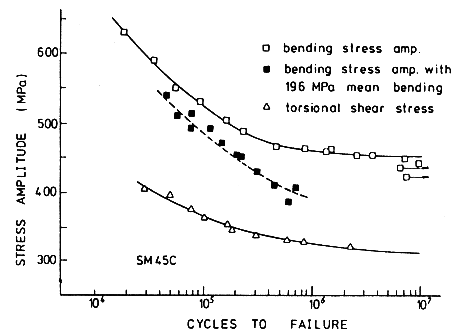
\includegraphics[width=0.8\textwidth]{figures//SM45C_SN.png} 
\caption{Fatigue curves made on SM45C steel by Lee \cite{lee2013out}}
\label{fig.SM45CSN}
\end{figure}


Preliminary fatigue tests were carried out under fully reversed bending and torsion separately.
\begin{table}[!h]
\centering
\begin{tabular}{|c|c|c|c|}
\hline
\begin{tabular}[c]{@{}c@{}}Bending Tests\\ (R=-1)\end{tabular}& \begin{tabular}[c]{@{}c@{}}N\\ {[}Cycles{]}\end{tabular} & \begin{tabular}[c]{@{}c@{}}$\sigma_{x,a}$\\ {[}MPa{]}\end{tabular} & \begin{tabular}[c]{@{}c@{}}$\sigma_{x,m}$\\ {[}MPa{]}\end{tabular}\\ \hline
1                                                                       & 1.9E4                                                             & 620                                                                    & 0                            \\ \hline
2                                                                       & 3.6E4                                                             & 590                                                                    & 0                              \\ \hline
3                                                                       & 5.8E4                                                             & 552                                                                     & 0                             \\ \hline
4                                                                       & 9E4                                                               & 535                                                                     & 0                             \\ \hline
5                                                                       & 1.7E5                                                             & 505                                                                       & 0                           \\ \hline
6                                                                       & 2.2E5                                                             & 490                                                                        & 0                          \\ \hline
7                                                                       & 4.4E5                                                             & 470                                                                         & 0                         \\ \hline
8                                                                       & 8E5                                                               & 465                                                                         & 0                         \\ \hline
9                                                                       & 1.4E6                                                             & 462                                                                         & 0                         \\ \hline
10                                                                      & 1.5E6                                                             & 465                                                                         & 0                         \\ \hline
11                                                                      & 2.4E6                                                             & 460                                                                         & 0                         \\ \hline
12                                                                      & 3.3E6                                                             & 460                                                                         & 0                         \\ \hline
13                                                                      & 6E6                                                               & 440                                                                          & 0                        \\ \hline
14                                                                      & 6.6E6                                                             & 458                                                                          & 0                        \\ \hline
15                                                                      & 7E6                                                               & 430                                                                          & 0                        \\ \hline
16                                                                      & 9E6                                                               & 448                                                                          & 0                        \\ \hline \hline
17                                                                      & 4.5E4                                                               & 540                                                                          & 196                        \\ \hline
18                                                                      & 5.4E4                                                               & 515                                                                          & 196                         \\ \hline
19                                                                      & 7E4                                                               & 520                                                                          & 196                         \\ \hline
20                                                                      & 7.1E4                                                               & 485                                                                          & 196                        \\ \hline
21                                                                      & 1.1E5                                                               & 485                                                                          & 196                       \\ \hline
22                                                                      & 1.5E5                                                               & 475                                                                          & 196                       \\ \hline
23                                                                      & 2E5                                                               & 460                                                                          & 196                      \\ \hline
24                                                                      & 2.1E5                                                               & 455                                                                          & 196                        \\ \hline
25                                                                      & 3E5                                                               & 435                                                                          & 196                       \\ \hline
26                                                                      & 4.3E5                                                              & 415                                                                          & 196                         \\ \hline
27                                                                      & 6.9E5                                                               & 410                                                                          & 196                         \\ \hline
28                                                                      & 5.8E5                                                               & 390                                                                          & 196                        \\ \hline
\end{tabular}
\caption{SM45C steel fully reversed bending tests(extracted from  \cite{lee2013out})}
\label{SM45Cbendingr1}
\end{table}

\begin{table}[!h]
\centering
\begin{tabular}{|c|c|c|}
\hline
\begin{tabular}[c]{@{}c@{}}Torsion Tests\\ (R=-1)\end{tabular} & \begin{tabular}[c]{@{}c@{}}N\\ {[}Cycles{]}\end{tabular} & \begin{tabular}[c]{@{}c@{}}$\tau_{xy,a}$\\ {[}MPa{]}\end{tabular} \\ \hline
1                                                                       & 2.9E4                                                             & 405                                                                                                \\ \hline
2                                                                       & 5E4                                                               & 399                                                                                                \\ \hline
3                                                                       & 7.8E4                                                             & 380                                                                                                \\ \hline
4                                                                       & 1E5                                                               & 365                                                                                                \\ \hline
5                                                                       & 1.8E5                                                             & 355                                                                                                \\ \hline
6                                                                       & 1.9E5                                                             & 349                                                                                                \\ \hline
7                                                                       & 3E5                                                               & 340                                                                                                \\ \hline
8                                                                       & 5.8E5                                                             & 335                                                                                                \\ \hline
9                                                                       & 8.2E5                                                             & 333                                                                                                \\ \hline
10                                                                      & 2.25E6                                                            & 325                                                                                                \\ \hline
\end{tabular}
\caption{SM45 steel fully reversed torsion tests(extracted from  \cite{lee2013out})}
\label{SM45CtorsionR1}
\end{table}



\begin{table}[!h]
\centering
\begin{tabularx}{\textwidth}{XXXXX}
\hline
\textbf{Group}               & \multicolumn{1}{l}{\textbf{\begin{tabular}[l]{@{}c@{}}N\\ {[}Cycles{]}\end{tabular}}} & \multicolumn{1}{l}{\textbf{\begin{tabular}[l]{@{}c@{}}$\tau_a$\\ {[}MPa{]}\end{tabular}}} & \multicolumn{1}{l}{\textbf{\begin{tabular}[l]{@{}c@{}}$\sigma_a$\\ {[}MPa{]}\end{tabular}}} & \multicolumn{1}{l}{\textbf{\begin{tabular}[l]{@{}c@{}}$\sigma_m$\\ {[}MPa{]}\end{tabular}}} \\ \hline
\multirow{10}{*}{\textbf{A}} & 29.9E3                                                                                & 282                                                                                       & 449                                                                                         & 0                                                                                           \\
& 35.7E3                                                                                & 334                                                                                       & 354                                                                                         & 0                                                                                           \\
& 50E3                                                                                  & 223                                                                                       & 485                                                                                         & 0                                                                                           \\
& 73.8E3                                                                                & 309                                                                                       & 357                                                                                         & 0                                                                                           \\
& 106E3                                                                                 & 217                                                                                       & 449                                                                                         & 0                                                                                           \\
& 106E3                                                                                 & 285                                                                                       & 370                                                                                         & 0                                                                                           \\
& 112E3                                                                                 & 199                                                                                       & 449                                                                                         & 0                                                                                           \\
& 131E3                                                                                 & 194                                                                                       & 457                                                                                         & 0                                                                                           \\
& 333E3                                                                                 & 252                                                                                       & 354                                                                                         & 0                                                                                           \\
& 431E3                                                                                 & 154                                                                                       & 437                                                                                         & 0                                                                                           \\ \hline
\multirow{10}{*}{\textbf{B}} & 53E3                                                                                  & 215                                                                                       & 441                                                                                         & 196                                                                                         \\
& 59.2E3                                                                                & 309                                                                                       & 286                                                                                         & 196                                                                                         \\
& 70.1E3                                                                                & 155                                                                                       & 464                                                                                         & 196                                                                                         \\
& 86.3E3                                                                                & 136                                                                                       & 473                                                                                         & 196                                                                                         \\
& 89.9E3                                                                                & 334                                                                                       & 173                                                                                         & 196                                                                                         \\
& 92.1E3                                                                                & 209                                                                                       & 403                                                                                         & 196                                                                                         \\
& 102E3                                                                                 & 177                                                                                       & 437                                                                                         & 196                                                                                         \\
& 135E3                                                                                 & 321                                                                                       & 167                                                                                         & 196                                                                                         \\
& 351E3                                                                                 & 179                                                                                       & 357                                                                                         & 196                                                                                         \\
& 394E3                                                                                 & 274                                                                                       & 182                                                                                         & 196                                                                                         \\ \hline
\end{tabularx}
\caption{With and without mean bending stress on out-of-phase($90^\circ$) fatigue of SM45C steel \cite{lee2013out}}
\label{meanSM45C}
\end{table}

In the case of multiaxial bending-torsion block tests(Table. \ref{meanSM45C}), we could alternatively adopt Von Mises stress as the value of $S_{a}$:
\begin{equation}
S_{a}=\sigma_{von}=\sqrt{\frac{1}{2}\left[ (\sigma_{xx}-\sigma_{yy})^2+(\sigma_{yy}-\sigma_{zz})^2+(\sigma_{zz}-\sigma_{xx})^2\right]+3(\tau_{xy}^2+\tau_{yz}^2+\tau_{zx}^2) }
\label{von}
\end{equation}

\newpage
\subsection{Identification of model parameters for steel SM45C}

We use the Von Mises yield strength combining the bending and torsion yield limits as $\sigma_y$. The fitted curve using experimental data in Table. \ref{meanSM45C} and data with mean stress effect is shown in \figref{fig.SM45C}b.
The tests on SM45C steel have illustrated that the mean bending stress has an influence on both uniaxial and multiaxial fatigue life. 

Although the uniaxial experimental data we extracted from Lee's curve \cite{lee2013out} of SM45C steel are slightly dispersed, we can find our model quite satisfactory in the case of SM45C steel. As for multiaxial 90 degree out of phase, fully reversed bending-torsion fatigue tests, our model is able to evaluate the cycles to failure.

\begin{table}[!h]
\centering
\begin{tabular}{|c|c|c|c|c|}
	\hline
	\textbf{$\beta$} & \textbf{$\lambda_+$} & \textbf{$\lambda_-$} & \textbf{$W_0$} & \textbf{$a$}  \\ \hline
	8    & 1 &0         &4.17E8 Pa  & 0.4    \\ \hline
\end{tabular}
\caption{Parameter identification of SM45C steel}
\label{sm45cpara}
\end{table}

\begin{Figure}[!h]{Calibration on  SM45C (\cite{lee2013out})}[fig.SM45C]
	\graphfile*[42]{figures//SM45C_bt1D_sn.png}[Bending and torsion test on SM45C steel(R=-1)]
	\graphfile*[42]{figures//SM45C_b1D_m_sn.png}[Bending test with mean stress on SM45C steel(R=-1,$\sigma_m=196 MPa$)]
	\\
	\graphfile*[42]{figures//SM45C_bt2D90_sn.png}[Bending-torsion 90 degree out-of-phase tests on SM45C steel]
	\graphfile*[42]{figures//SM45C_bt2D90_m_sn.png}[Bending-torsion 90 degree out-of-phase with mean stress tests on SM45C steel]
\end{Figure}

\begin{Figure}[!h]{Calibration on  SM45C (\cite{lee2013out})}[fig.SM45C]
\graphfile*[42]{figures//SM45C_bt1D_err.png}[Bending and torsion test on SM45C steel(R=-1)]
\graphfile*[42]{figures//SM45C_b1D_m_err.png}[Bending test with mean stress on SM45C steel(R=-1,$\sigma_m=196 MPa$)]
\\
\graphfile*[42]{figures//SM45C_bt2D90_err.png}[Bending-torsion 90 degree out-of-phase tests on SM45C steel]
\graphfile*[42]{figures//SM45C_bt2D90_m_err.png}[Bending-torsion 90 degree out-of-phase with mean stress tests on SM45C steel]
\end{Figure}


\clearpage
\section{Experimental validation of the model on 10 HNAP steel}
\subsection{Presentation of the material}
Fatigue tests were performed on the HNAP steel. It is a very low carbon steel
which resembles the 10 CN 6. In Table.\ref{tab.10HNAPchem}, its chemical composition is given:	
\begin{table}[!h]
\centering
\begin{tabular}{rrrrrrrrr}
\hline
C      & Mn     & Si     & P      & S      & Cr     & Cu     & Ni     & Fe       \\
0.12\% & 0.71\% & 0.41\% & 0.08\% & 0.03\% & 0.81\% & 0.30\% & 0.50\% & the rest \\ \hline
\end{tabular}
\caption{Chemical composition of 10 HNAP steel\cite{Bedkowski1994}}
\label{tab.10HNAPchem}
\end{table}
The mechanical properties of this steel are given in Table.\ref{tab.10HNAPmec}:
\begin{table}[!h]
\centering
\begin{tabular}{rrrrr}
\hline
$Re_{0.2\%}$ & $R_m$   & A    & $\nu$ & E          \\
418 MPa     & 566 Mpa & 32\% & 0.29  & 215000 Mpa \\ \hline
\end{tabular}
\caption{Mechanical characteristics of steel 10 HNAP\cite{Bedkowski_1994}}
\label{tab.10HNAPmec}
\end{table}

where 
\begin{table}[!h]
\centering
\begin{tabular}{ll}
$Re_{0.2\%}$ & : elastic limit at 0.2\% of plastic deformation, \\
$R_m$      & : maximum tensile strength,                                                                  \\
A          & : elongation at break,                                                                       \\
$\nu$      & : Poisson's coefficient,                                                                     \\
E          & : Young's modulus.                                                                          
\end{tabular}
\end{table}

\subsection{Description of fatigue tests on 10 HNAP steel}
The Macha team performed a large number of fatigue tests on the HNAP steel. Thus, it performed not only simple tensile compression and torsion tests (R = -1) in order to establish The corresponding Wöhler curves but also tests under variable loading on cylindrical specimens of the same material\cite{ACHTELIC1994}. VIDAL\cite{VIDAL1996} carried out tensile tests on this material for various mean stress values. It has established the Wöhler curve in repeated traction in order to validate on this steel the method of Robert whose use requires three Wöhler curves in symmetrical alternating traction, symmetrical alternating torsion and repetitive traction.

\vspace{6pt}
\noindent
\textbf{Wöhler curve in tension-compression}

The model chosen by Macha and recovered by Jabbado\cite{jabbado:pastel-00002116} for the tensile-compression Wöhler curve is that of Basquin:
\begin{equation}
lnN=68.361 − 9.82ln\left( \sigma_{-1}\right) 
\end{equation}

\noindent
\textbf{Wöhler curve in symmetrical alternating torsion}

The symmetric alternating torsion Wöhler curve was recovered by Jabbado\cite{jabbado:pastel-00002116} using following equation:
\begin{equation}
lnN=21.55 − 0.0385\tau_{-1}
\end{equation}

\noindent
\textbf{Tensile fatigue tests for various mean stress values}

VIDAL\cite{VIDAL1996} carried out tensile tests on HNAP steel for various values of mean stress. The results are summarized in Table.\ref{tab.10HNAPmean}. They allowed us to plot the Wöhler curves for different values of the mean stress $\sigma_m$. These curves are modeled by the Wöhler equation:
\begin{equation}
lnN=A − B\sigma_{max}
\label{eq.10HNAPmean}
\end{equation}
In the Table.\ref{tab.10HNAPAB}, the values of the constants A and B of Eq.\eqref{eq.10HNAPmean}.
\begin{table}[!h]
\centering
\begin{tabular}{ccl}
\hline
\multicolumn{1}{l}{$\sigma_a$(MPa)} & \multicolumn{1}{l}{$\sigma_m$(MPa)} & $N_{exp}$(cycles)    \\ \hline
250                                 & 75                                  & 439300;402500        \\
270                                 & 75                                  & 358200;854700;318700 \\
290                                 & 75                                  & 252300;376300;379700 \\
310                                 & 75                                  & 54800;123400;45000   \\ \hline
250                                 & 150                                 & 157400;1333000       \\
270                                 & 150                                 & 172100;121500;233100 \\
290                                 & 150                                 & 124300;41900;60500   \\ \hline
230                                 & 225                                 & 413900;204500;545200 \\
250                                 & 225                                 & 122400;229600;104000 \\
270                                 & 225                                 & 110000;29900;66000   \\ \hline
190                                 & 300                                 & 497100;234300;524800 \\
210                                 & 300                                 & 463500;367300;259500 \\
230                                 & 300                                 & 219000;179400;222400 \\
250                                 & 300                                 & 95300;118200;59100   \\ \hline
\end{tabular}
\caption{Experimental results of tensile tests for various values of $\sigma_m$}
\label{tab.10HNAPmean}
\end{table}

\noindent
\textbf{Fatigue testing under variable loading}

Random multiaxial loading fatigue tests were performed on cylindrical HNAP steel specimens\cite{ACHTELIC1994}. The load considered is proportional and results from a combination of bending and torsion. The random signal is stationary and has a normal distribution as a probability distribution. Tests of this type have been analyzed and simulated by Carpinteri et al.\cite{carpinteri2003multiaxial}. They were provided to us in the form of tests carried out on the HNAP steel for two values of the angle $\alpha'$: $\alpha' = \pi / 8$ and $\alpha' = \pi / 4$ . $\alpha' $ is the angle made by the resultant moment $M$ with the bending moment $M_B$ (see \figref{fig.10HNAPsample}).

\begin{figure}[!h]
\centering
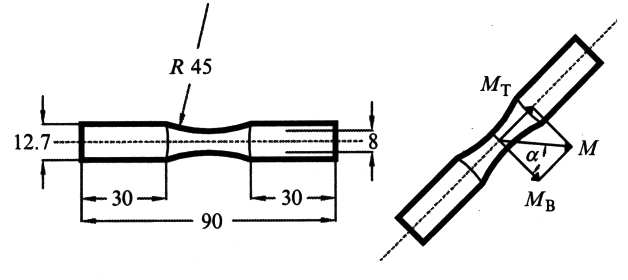
\includegraphics[width=0.7\textwidth]{figures//10HNAPsample.png} 
\caption{Bending-torsion fatigue tests on cylindrical specimens\cite{carpinteri2003multiaxial}}
\label{fig.10HNAPsample}
\end{figure}

The stationary random loading sequence contains 49152 values recorded by a time interval of 0.00375 seconds (frequency = 266.67 Hz). It is shown in \figref{fig.10HNAPrandom}. Its total duration is 184.32 seconds. This sequence is multiplied by load coefficients corresponding to bending $f (\sigma_{xx})$ and torsion $f (\tau_{xy})$ in order to obtain random multiaxial loading sequences. As the signal is stationary, the breaking life is determined in terms of number of sequences with break $N_{Sq}$. Knowing $N_{Sq}$ and the total time in seconds of the sequence studied, it is easy to express the lifetime of the piece in seconds. The results of fatigue tests under variable loads are summarized in Table.\ref{tab.10HNAPrand1} and Table.\ref{tab.10HNAPrand2} as a function of angle $\alpha'$ and ratio r; $r =f(\tau_{xy})/f(\sigma_{xx})$.
\begin{figure}[!h]
\centering
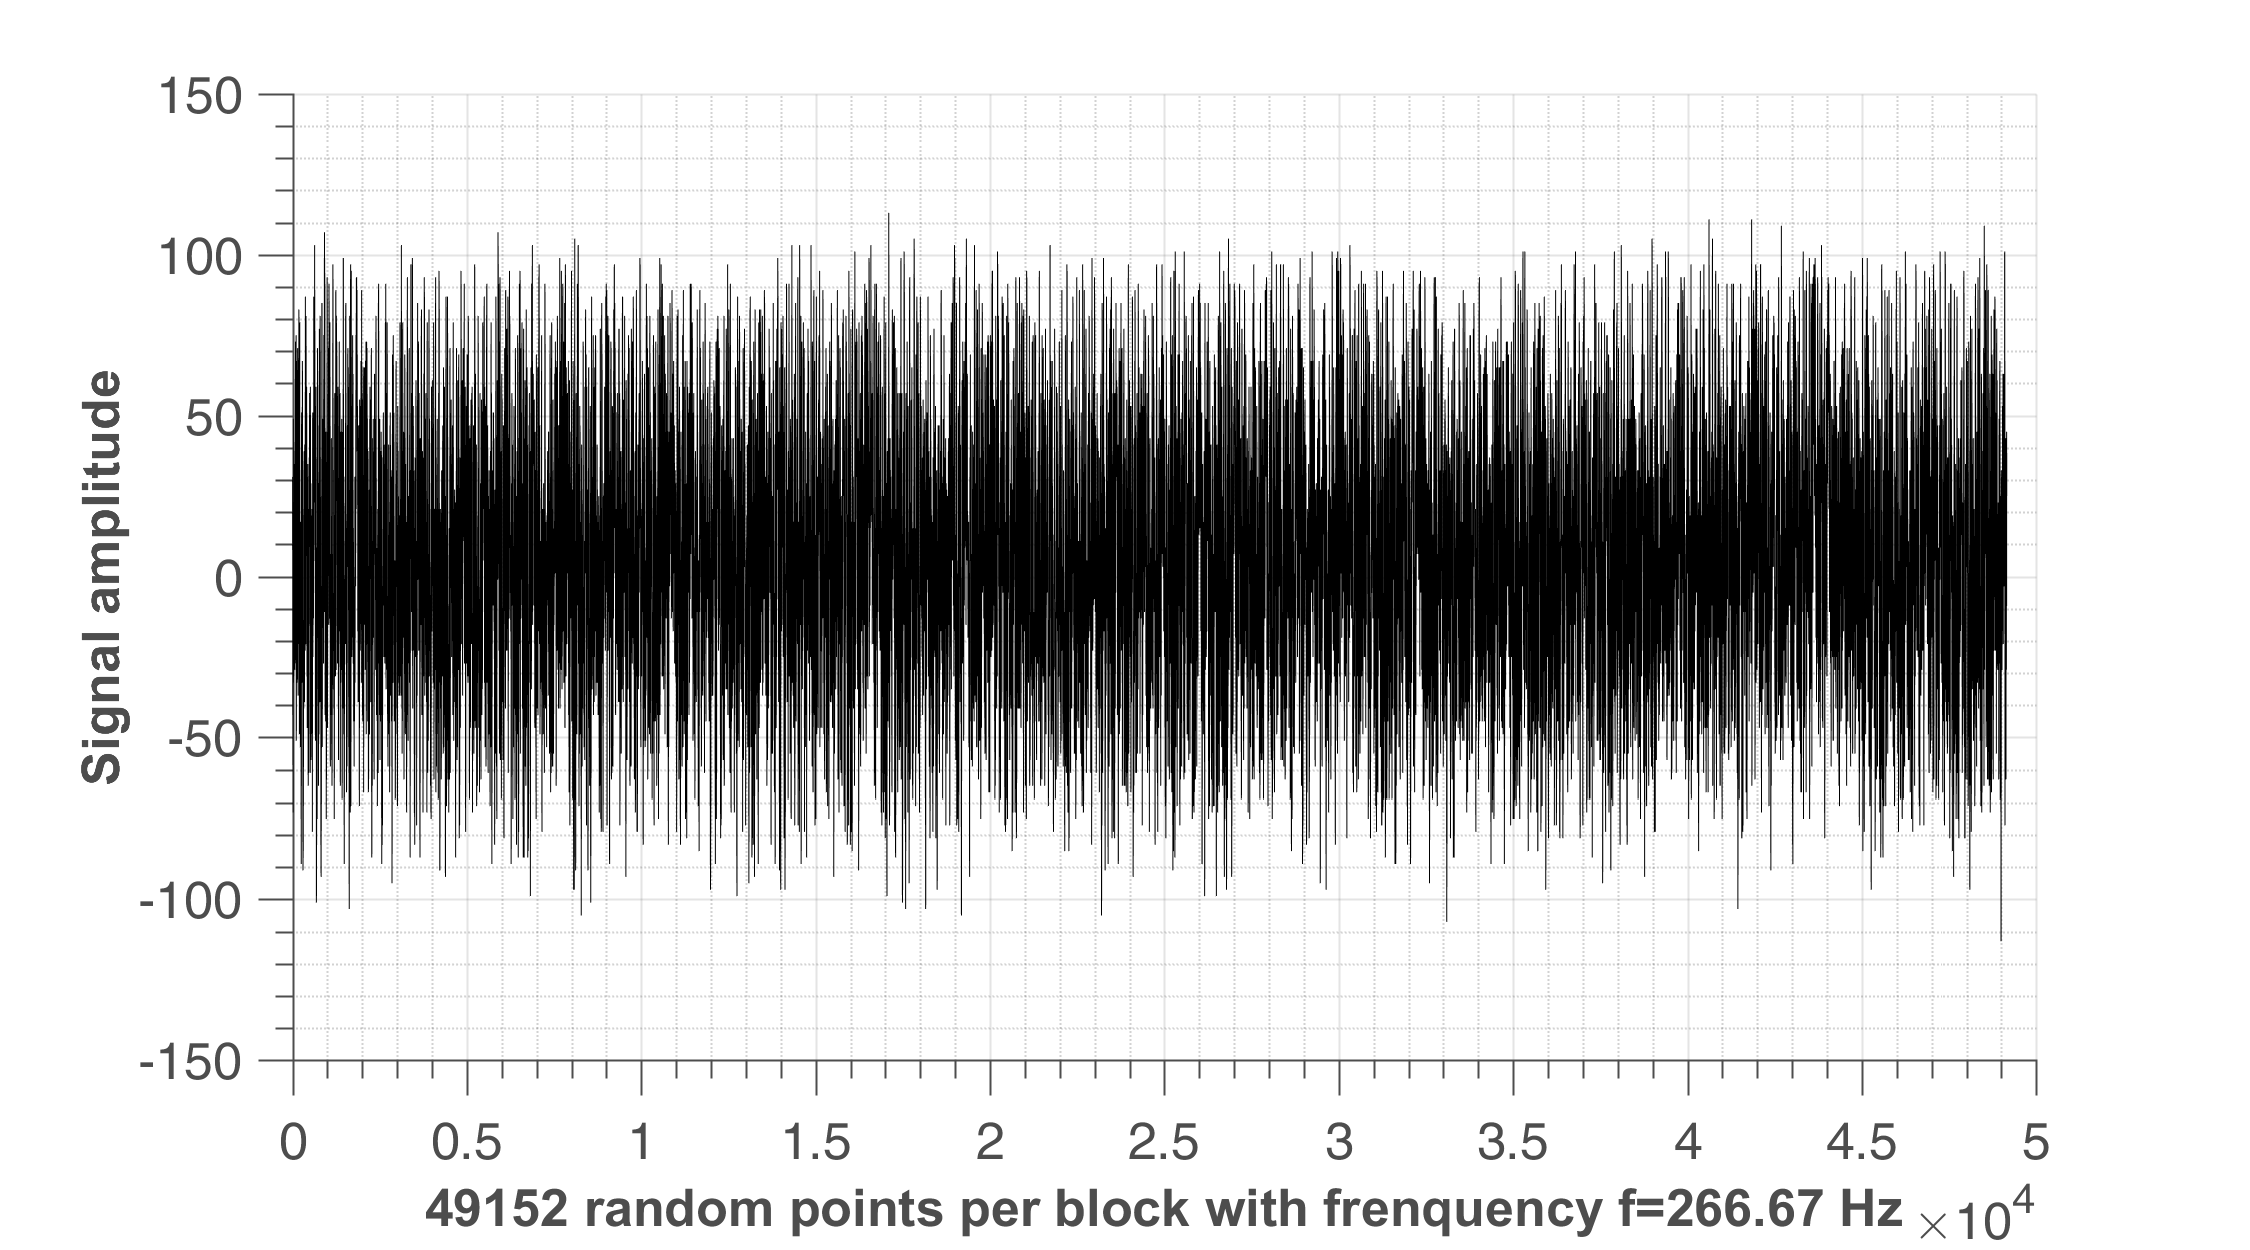
\includegraphics[width=\textwidth]{figures//10HNAPrandomblock.png} 
\caption{Bending-torsion fatigue tests on cylindrical specimens\cite{carpinteri2003multiaxial}}
\label{fig.10HNAPrandom}
\end{figure}

\textbf{1st type of tests:} $\alpha' = \pi / 8$ and $r =f(\tau_{xy})/f(\sigma_{xx})=0.2$.

\begin{table}[!h]
\centering
\begin{tabular}{lrrrr}
\hline
$N^o$ & $f(\sigma_{xx})$ & $f(\tau_{xy})$ & $r$   & $T_{exp}(s)$ \\ \hline
1     & 5.7084                  & 1.1822  & 0.2 & 16843.2    \\
2     & 5.2917                  & 1.0959  & 0.2 & 17780.1    \\
3     & 4.8337                  & 1.0010  & 0.2 & 24416.5    \\
4     & 5.2674                  & 1.0909  & 0.2 & 24858.2    \\
5     & 5.4534                  & 1.1294  & 0.2 & 26518.3    \\
6     & 5.2002                  & 1.0769  & 0.2 & 36162.3    \\
7     & 4.7944                  & 0.9929  & 0.2 & 47600.4    \\
8     & 4.3862                  & 0.9084  & 0.2 & 57993.9    \\
9     & 4.6241                  & 0.9576  & 0.2 & 60428      \\
10    & 4.0194                  & 0.8324  & 0.2 & 73373.3    \\
11    & 4.0127                  & 0.8310  & 0.2 & 87609.1    \\
12    & 4.2292                  & 0.8758  & 0.2 & 89185.2    \\
13    & 3.9213                  & 0.8121  & 0.2 & 106900     \\
14    & 3.7731                  & 0.7814  & 0.2 & 117358     \\
15    & 4.1148                  & 0.8521  & 0.2 & 118902     \\
16    & 3.6150                  & 0.7486  & 0.2 & 132448     \\
17    & 3.3135                  & 0.6862  & 0.2 & 170571     \\
18    & 4.1298                  & 0.8553  & 0.2 & 178215     \\
19    & 3.4761                  & 0.7199  & 0.2 & 225288     \\
20    & 3.3430                  & 0.6923  & 0.2 & 352635     \\
21    & 3.0135                  & 0.6241  & 0.2 & 355720     \\ \hline
\end{tabular}
\caption{Fatigue results under variable loads for $\alpha' = \pi / 8$ and $r =f(\tau_{xy})/f(\sigma_{xx})=0.2$}
\label{tab.10HNAPrand1}
\end{table}

\textbf{2nd type of tests:} $\alpha' = \pi / 4$ and $r =f(\tau_{xy})/f(\sigma_{xx})=0.5$.

\begin{table}[]
\centering
\begin{tabular}{lrrrr}
\hline
$N^o$ & $f(\sigma_{xx})$ & $f(\tau_{xy})$ & $r$   & $T_{exp}(s)$ \\ \hline
1   & 4.2519                  & 2.126   & 0.5 & 15379.4    \\
2   & 4.0567                  & 2.0284  & 0.5 & 21465.7    \\
3   & 3.8982                  & 1.9491  & 0.5 & 25350.4    \\
4   & 3.7823                  & 1.8912  & 0.5 & 45949      \\
5   & 3.5963                  & 1.7982  & 0.5 & 62434.8    \\
6   & 3.4497                  & 1.7249  & 0.5 & 75225.7    \\
7   & 2.9423                  & 1.4712  & 0.5 & 115009     \\
8   & 2.8814                  & 1.4407  & 0.5 & 136794     \\
9   & 2.3299                  & 1.165   & 0.5 & 203365     \\
10  & 2.8399                  & 1.42    & 0.5 & 221370     \\
11  & 2.8493                  & 1.4247  & 0.5 & 244757     \\
12  & 2.2542                  & 1.1271  & 0.5 & 251723     \\
13  & 2.3651                  & 1.1826  & 0.5 & 288080     \\
14  & 2.4215                  & 1.2108  & 0.5 & 405444     \\ \hline
\end{tabular}
\caption{Fatigue results under variable loads for $\alpha' = \pi / 4$ and $r =f(\tau_{xy})/f(\sigma_{xx})=0.5$}
\label{tab.10HNAPrand2}
\end{table}

In \figref{fig.10HNAP2Drandom}, an example of a random multiaxial loading sequence is given.
\begin{figure}[!h]
\centering
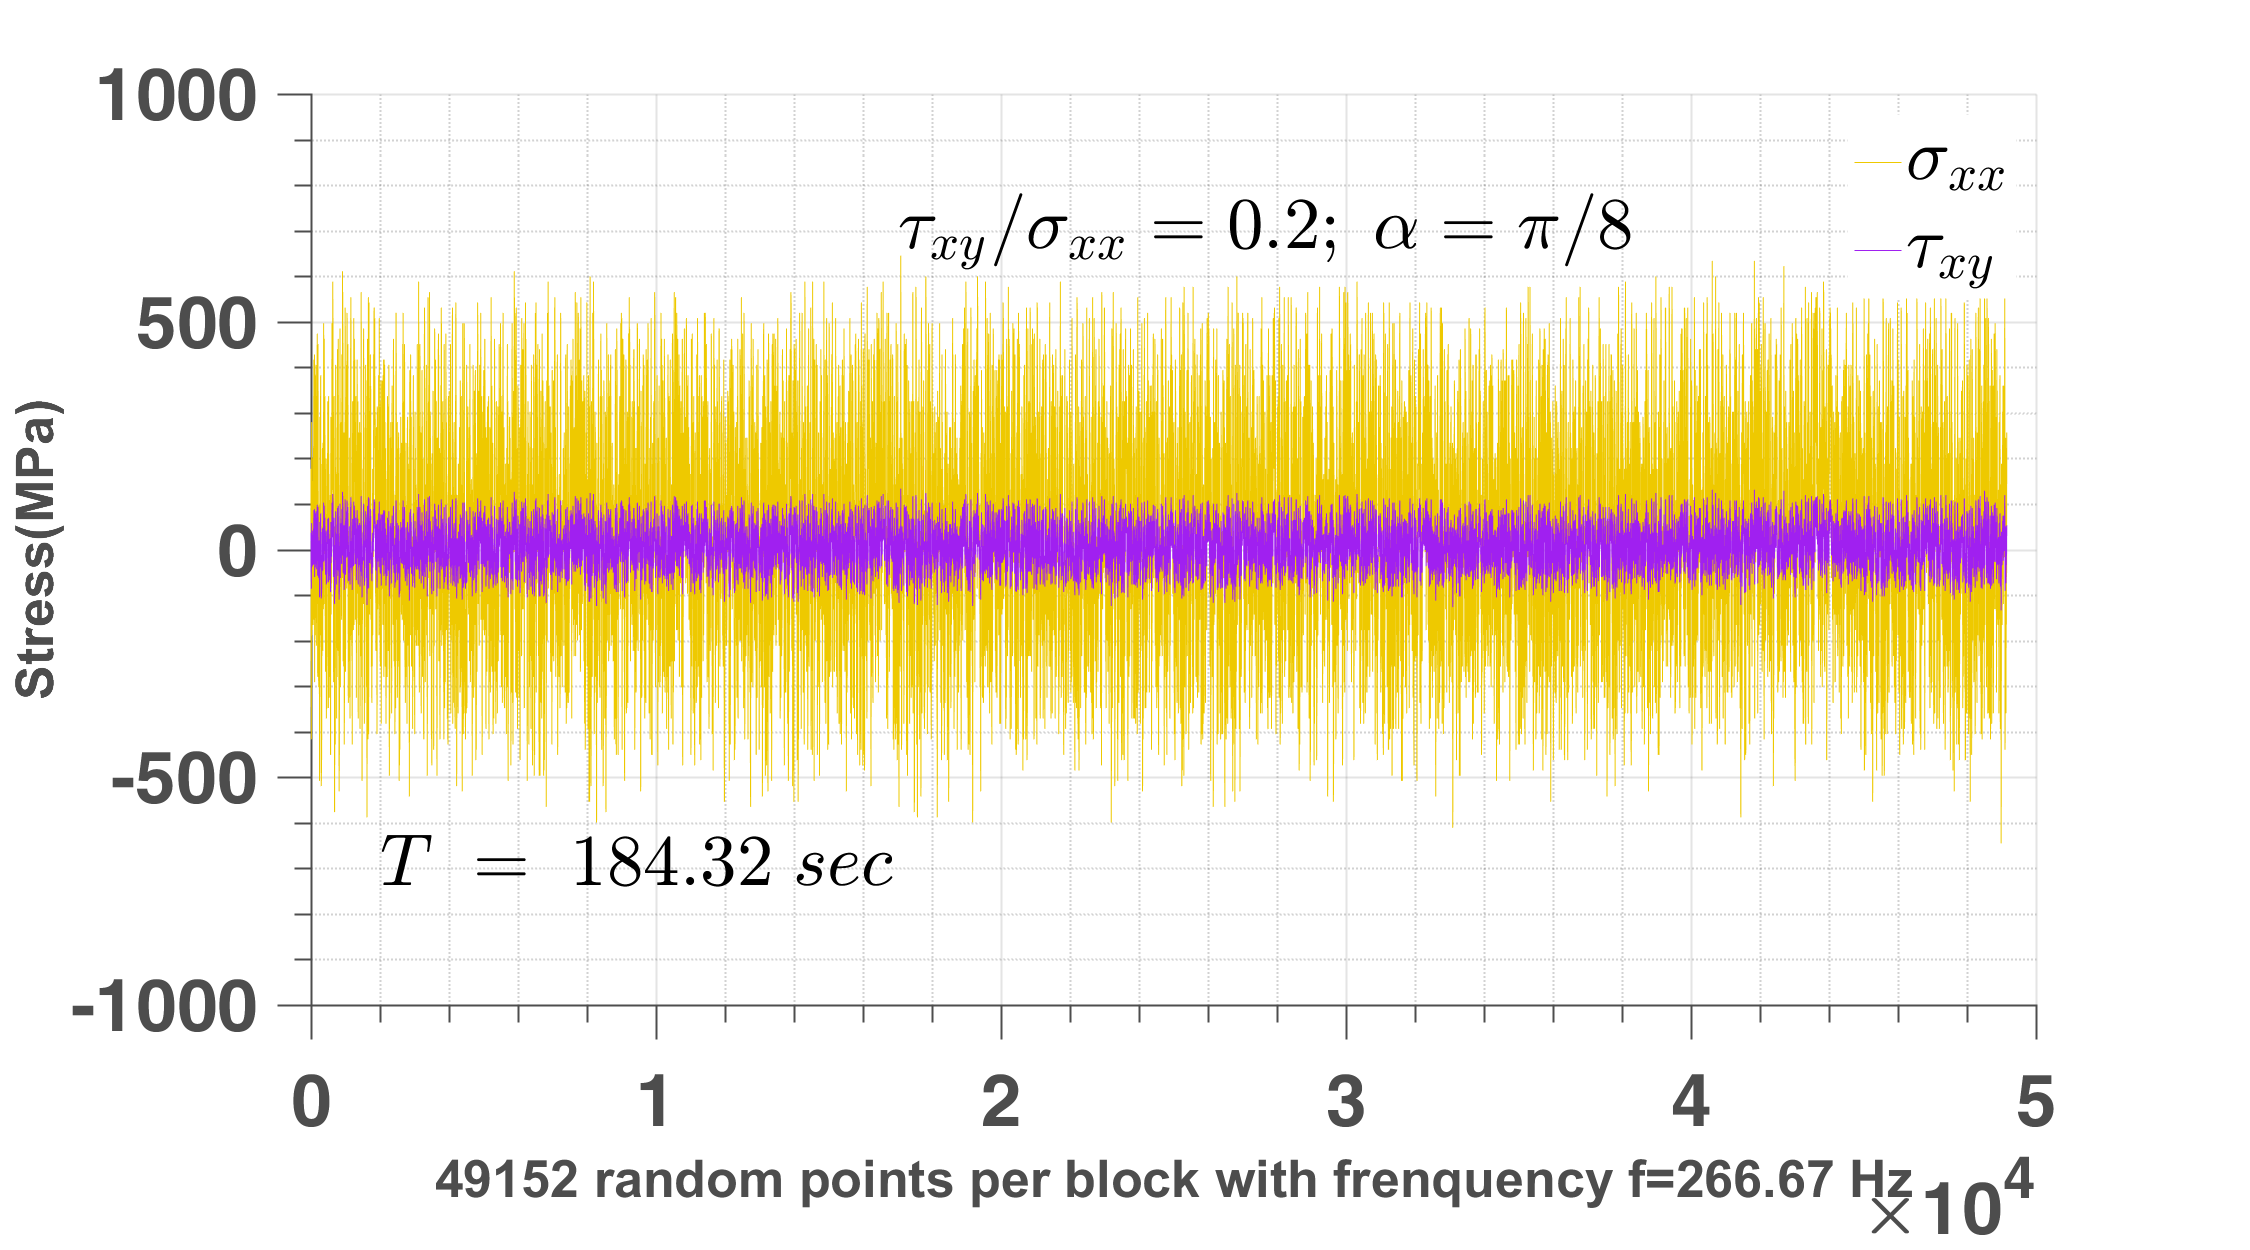
\includegraphics[width=\textwidth]{figures//HNAP_random.png} 
\caption{Multiaxial random loading sequence}
\label{fig.10HNAP2Drandom}
\end{figure}

\subsection{Identification of model parameters of 10HNAP steel}
As mentioned earlier, the identification of the model parameters requires a Wöhler curve. This initiates the value of $\beta$, in the mean stress tests we have got the value of $\lambda$. And the value of $W_0$ and a comes from random loading. The parameters of the HNAP steel model can be identified by referring to Table.\ref{tab.10HNAP.para}. They are grouped in the following table:
\begin{table}[!h]
\centering
\begin{tabular}{|c|c|c|c|c|}
	\hline
	\textbf{$\beta$} & \textbf{$\lambda_+$} & \textbf{$\lambda_-$} & \textbf{$W_0$} & \textbf{$a$}  \\ \hline
	5.34    & 1.7 &0         &6.48E8 Pa  & 0.4    \\ \hline
\end{tabular}
\caption{Model parameters for 10HNAP steel}
\label{tab.10HNAP.para}
\end{table}

\subsection{Simulation of fatigue tests performed on 10HNAP steel}
After determining the parameters of the HNAP steel model and calculated pcs for each of the tests tested, the number of priming cycles can be obtained by directly applying equation \eqref{eq.cycNF} for the proportional periodic loads of constant amplitude and for multiaxial loadings of variable amplitude.
\begin{figure}[!h]
	\centering
	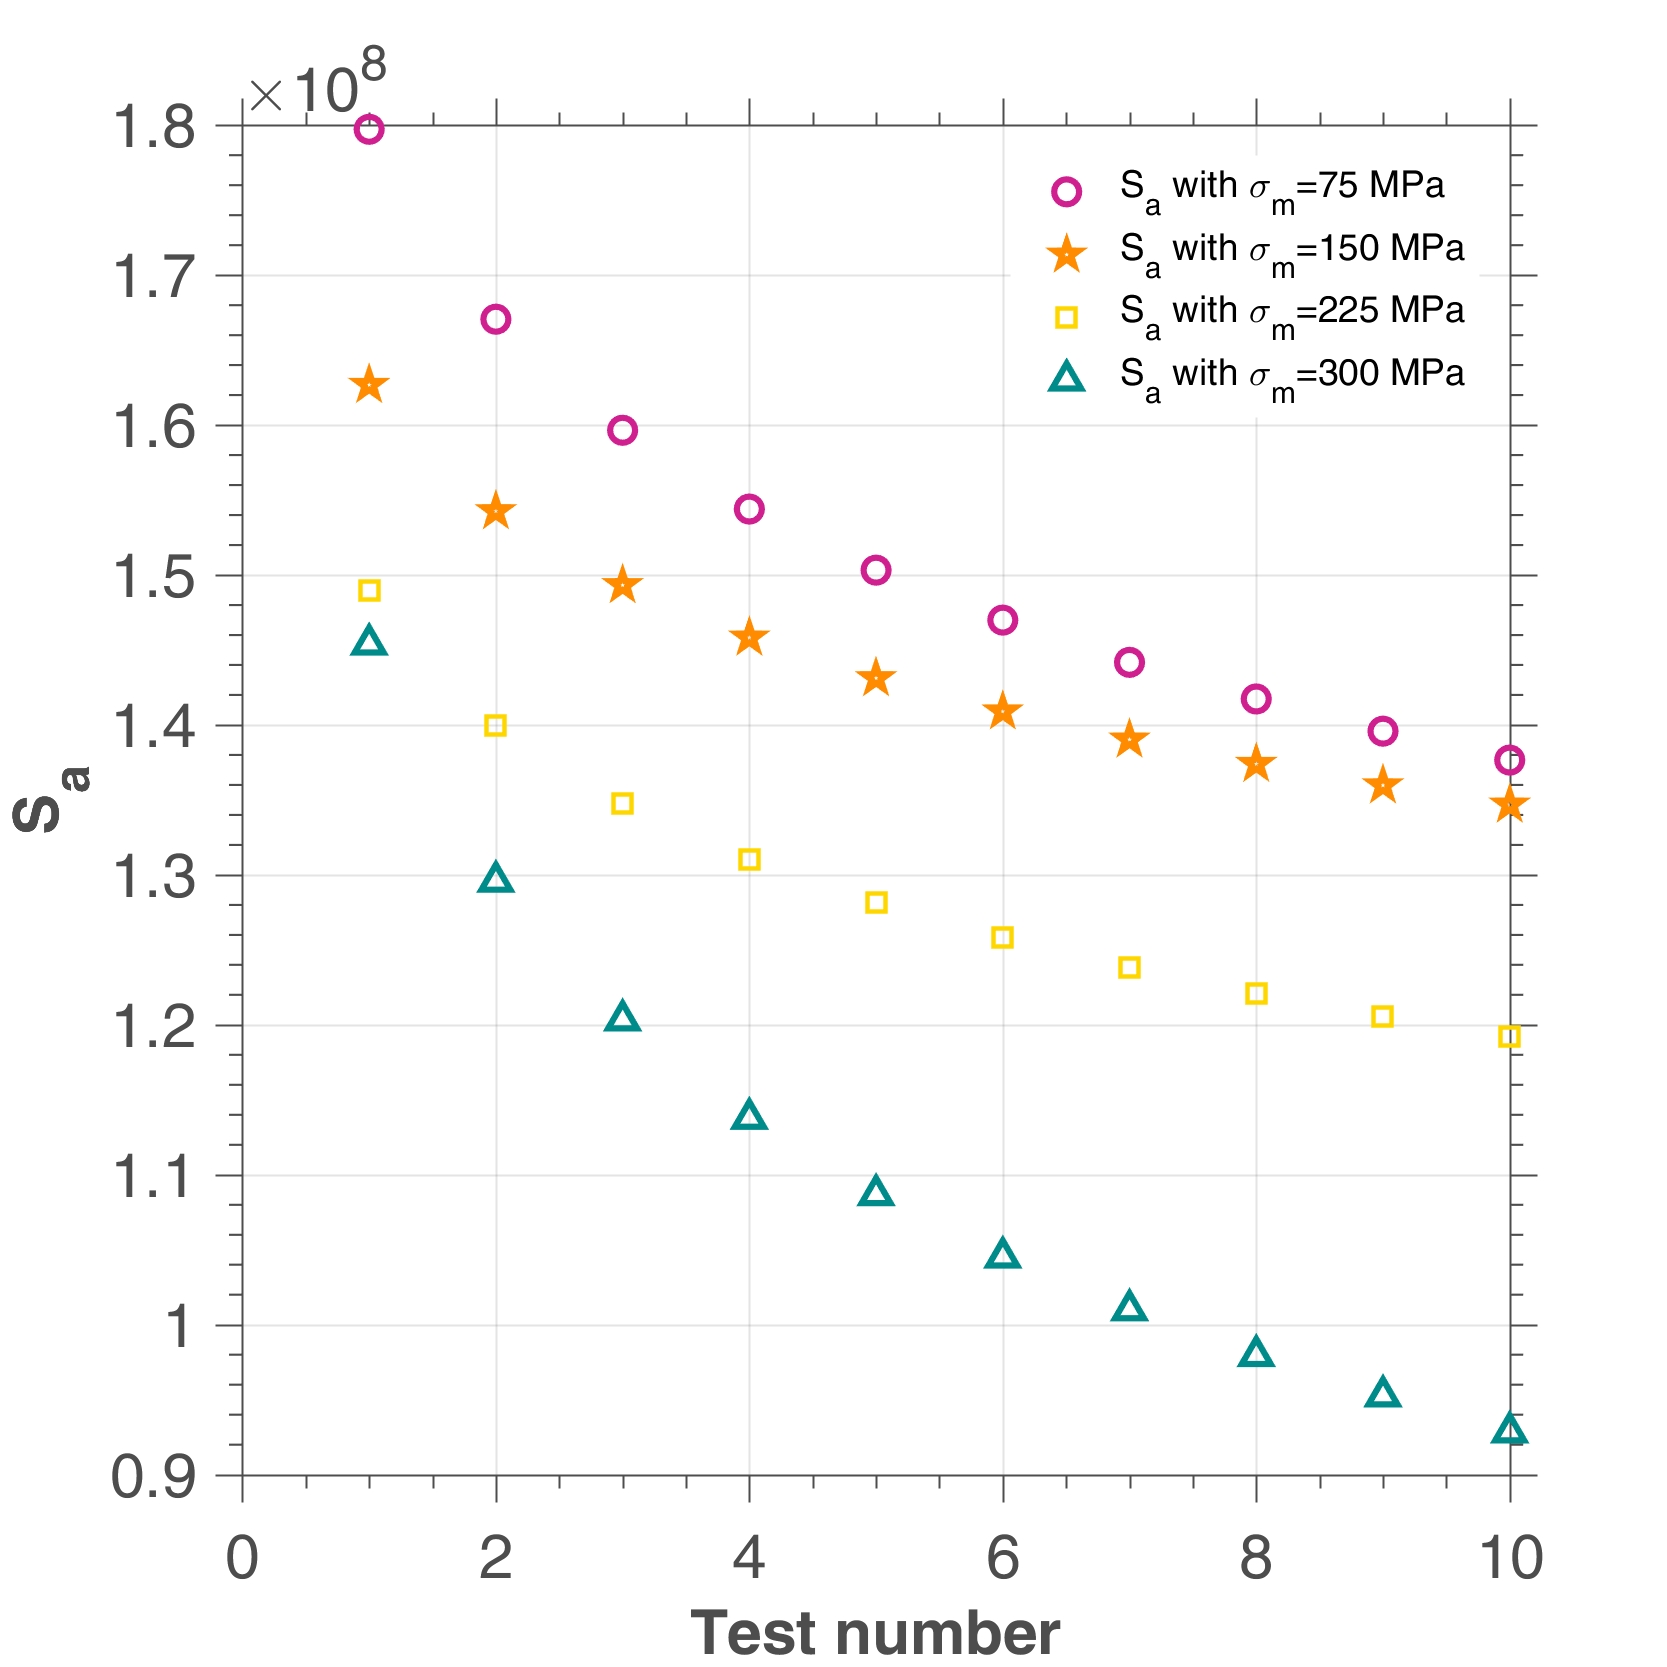
\includegraphics[width=\textwidth]{figures//10HNAP_b1D_m_Smax.png} 
	\caption{$S_{a}$ of bending tests with mean stress on 10HNAP}
	\label{fig.10HNAPSmax}
\end{figure}
\begin{figure}[!h]
	\centering
	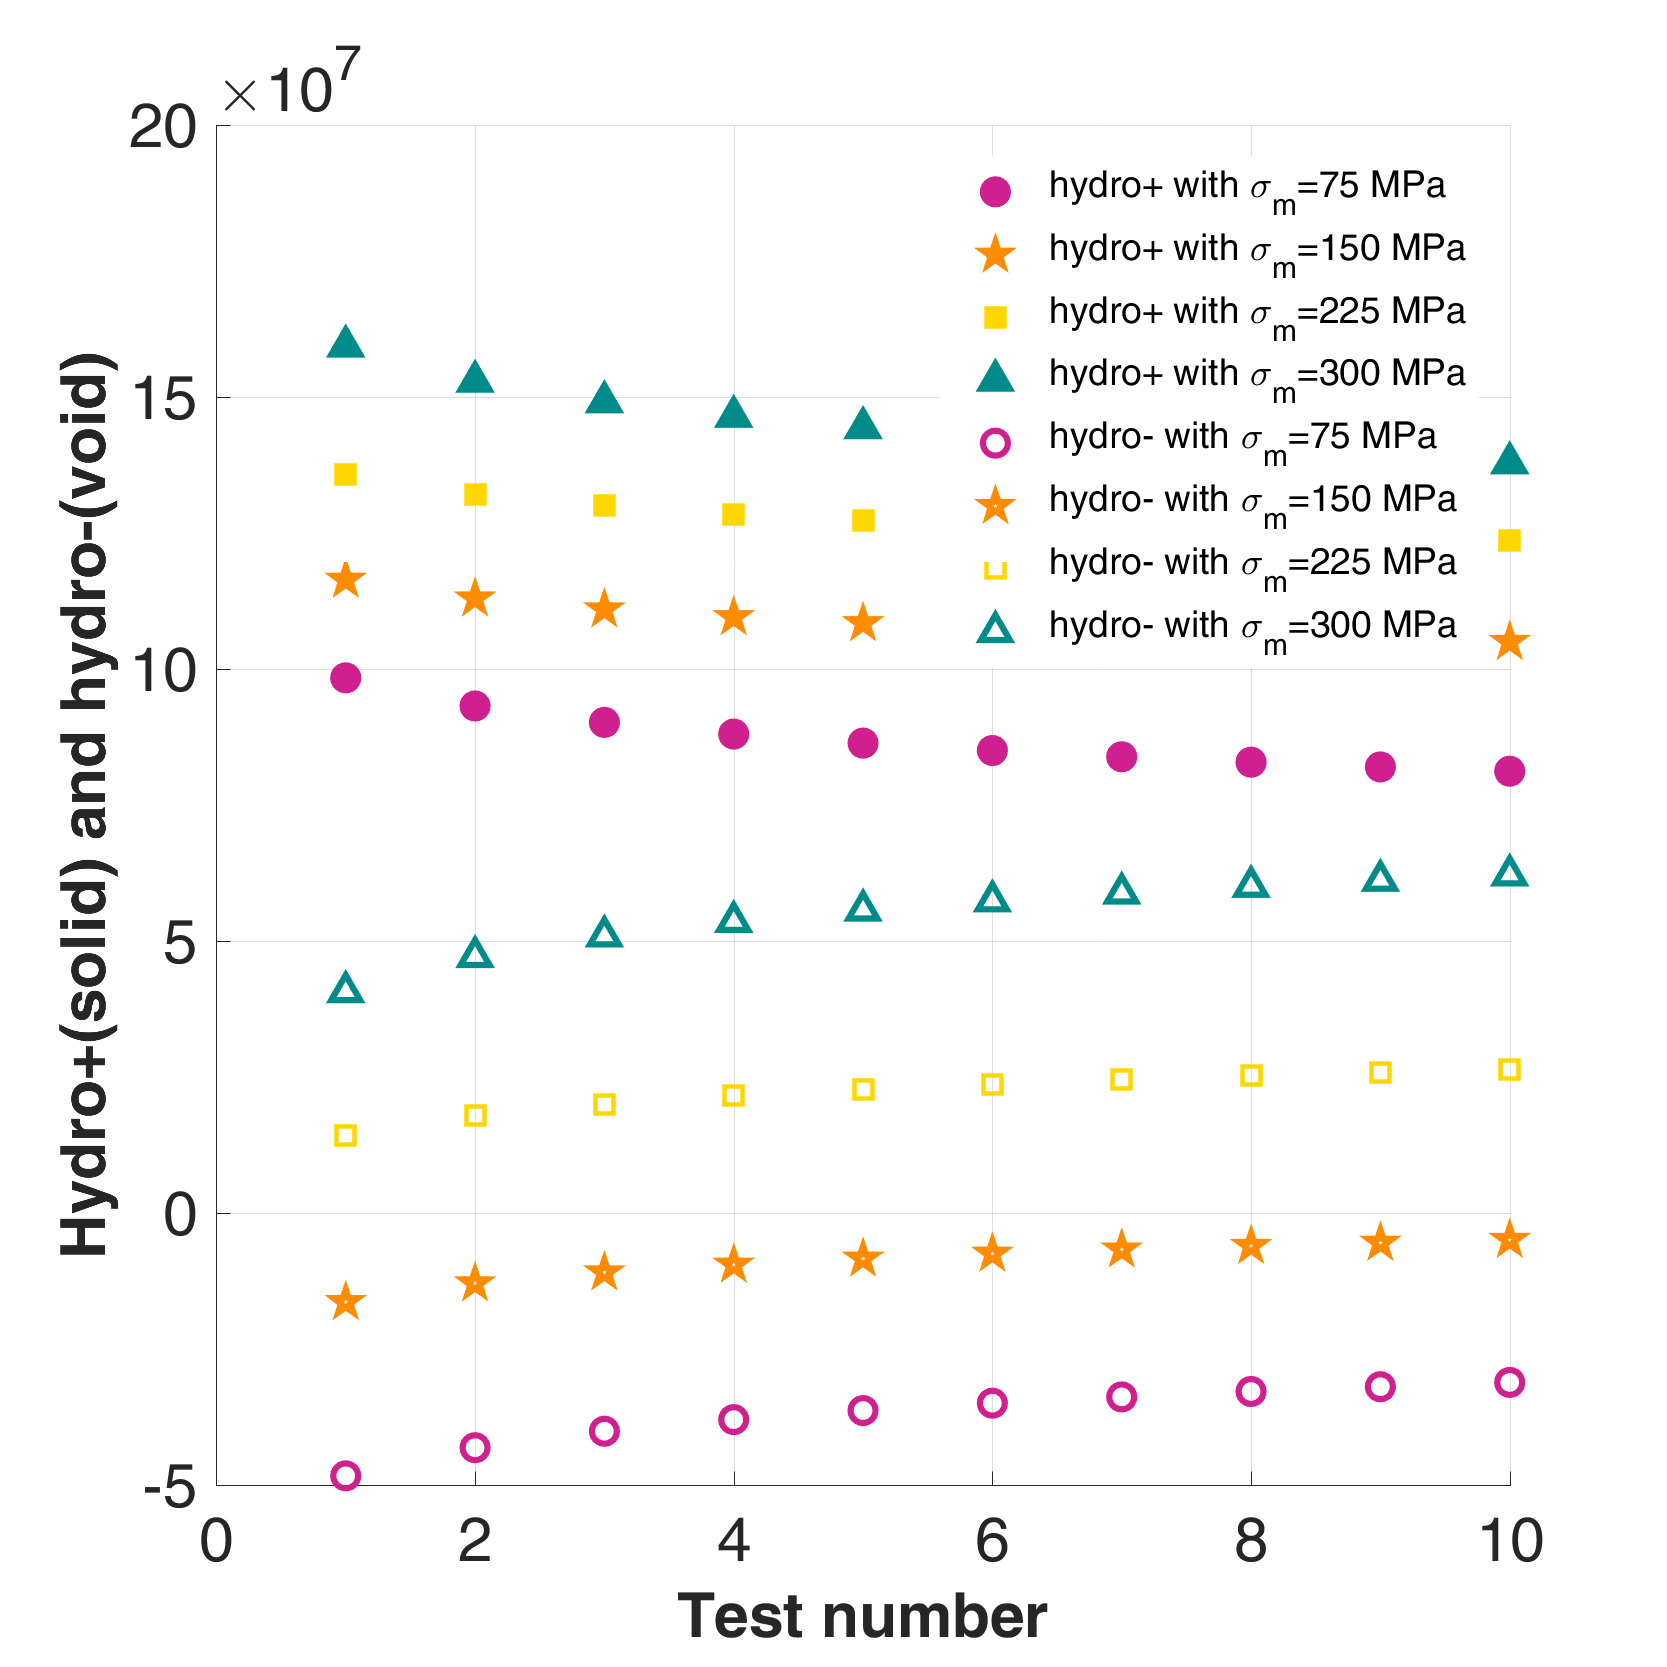
\includegraphics[width=\textwidth]{figures//10HNAP_b1D_m_hydro.png} 
	\caption{$Hydro_{+-}$ of bending tests with mean stress on 10HNAP}
	\label{fig.10HNAPhydro}
\end{figure}

In \figref{fig.10HNAP1} and \figref{fig.10HNAP2}, we give the prediction results of the torsion tests used to identify $\beta$ and $W_0$ of the model, then we use the bending with various mean stress to get the parameter $\lambda$. These are to be taken with caution because of the effect of the gradient because the specimens stressed in tension and in torsion are not of the same nature.
%%-------------S_eq vs NF----------------------------
\begin{figure}[!h]
	\centering
	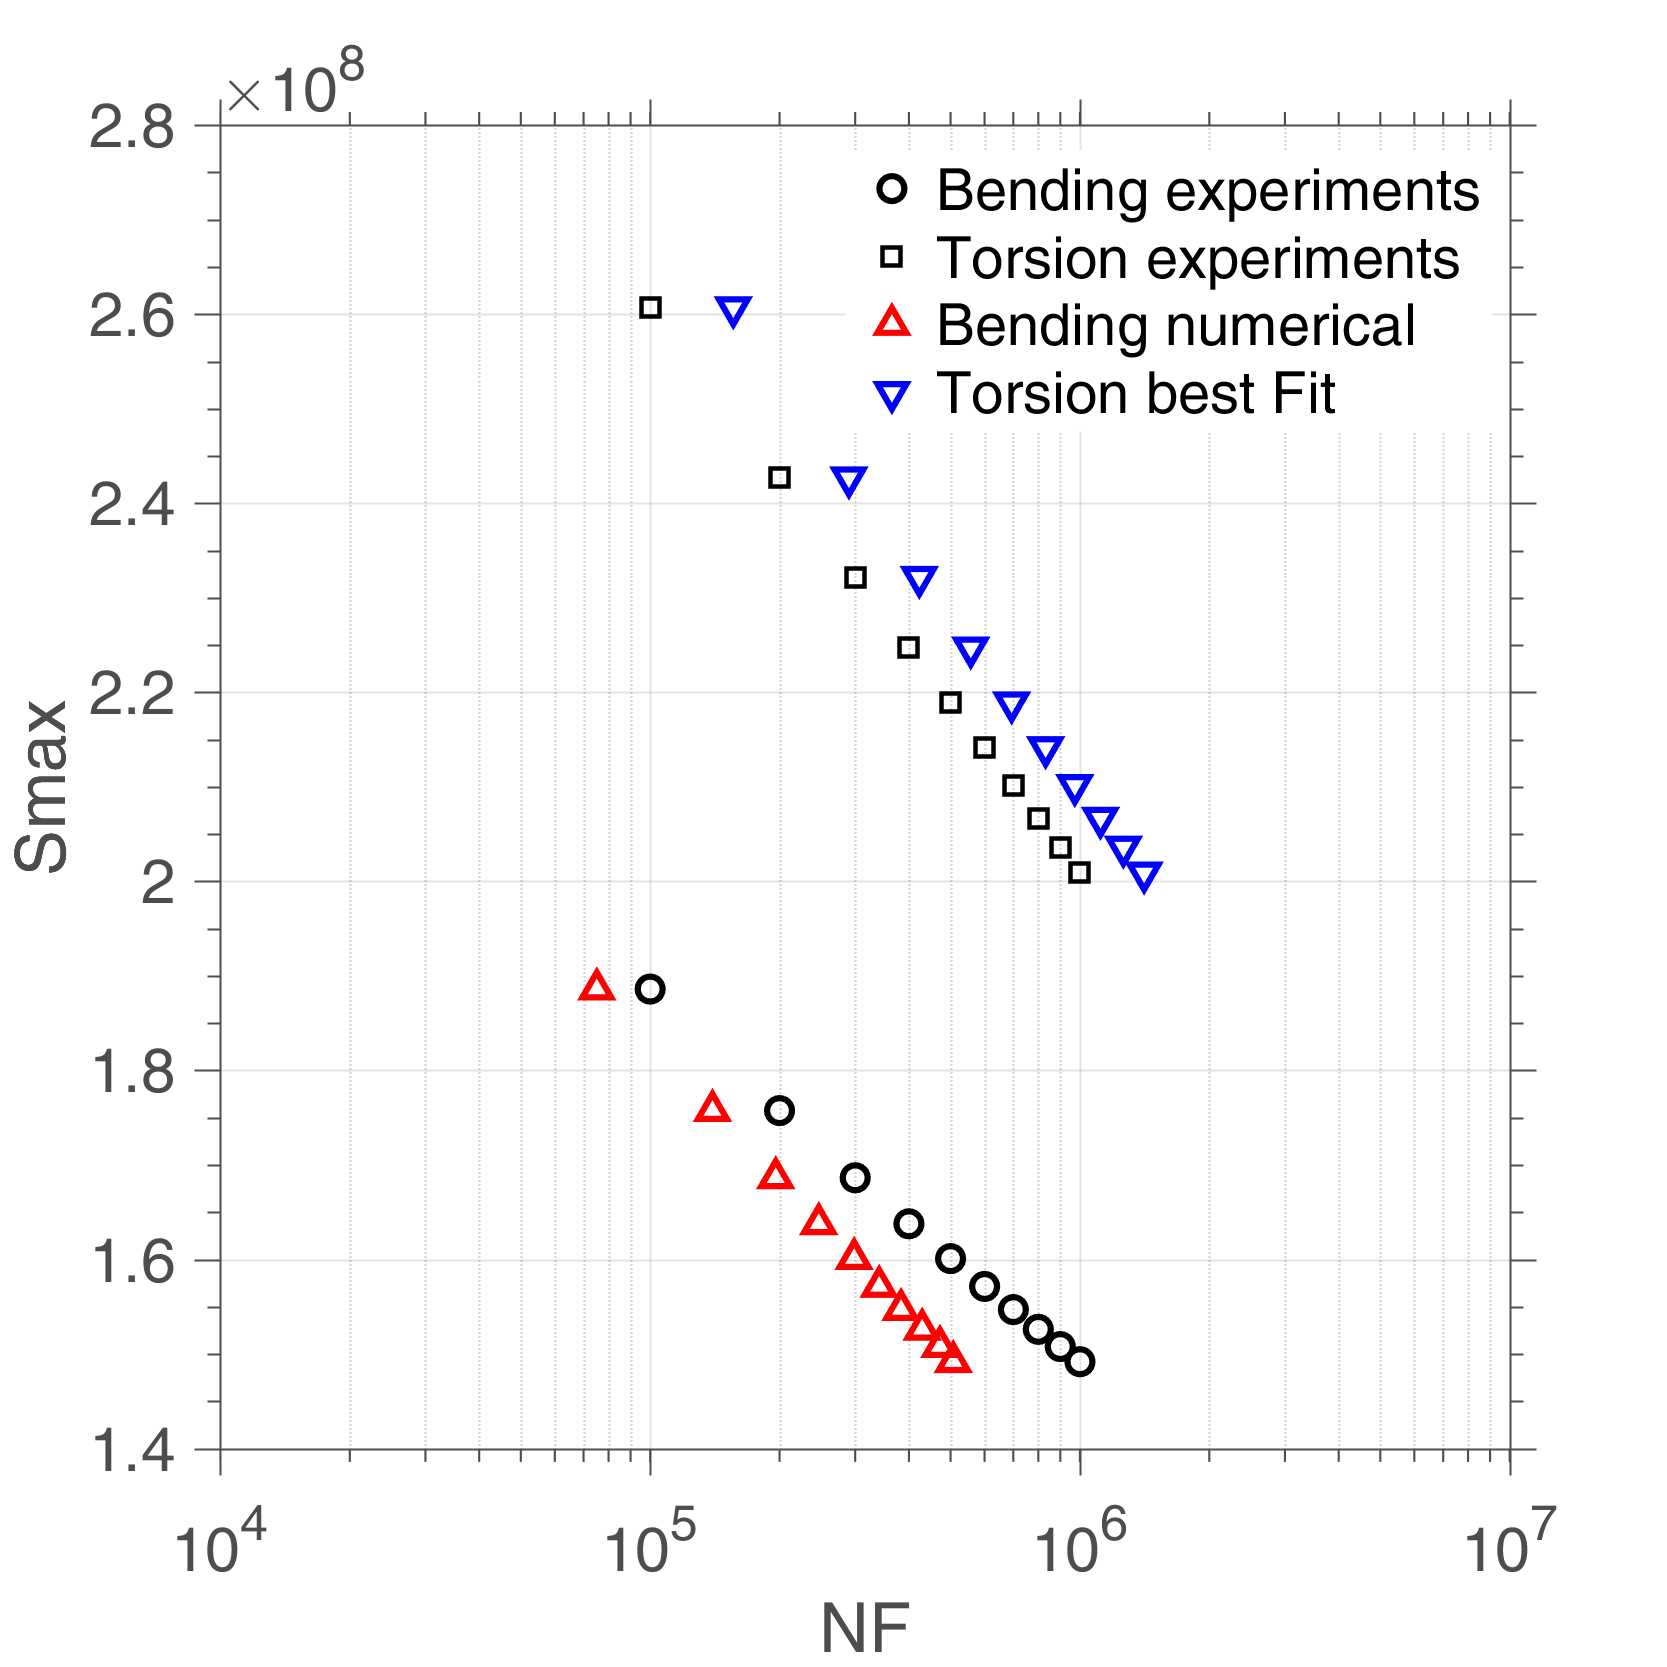
\includegraphics[width=\textwidth]{figures//10HNAP_bt1D_sn.png} 
	\caption{Bending and torsion test on 10HNAP steel(R=-1)}
	\label{fig.bt1D10HNAPsn}
\end{figure}
\begin{figure}[!h]
	\centering
	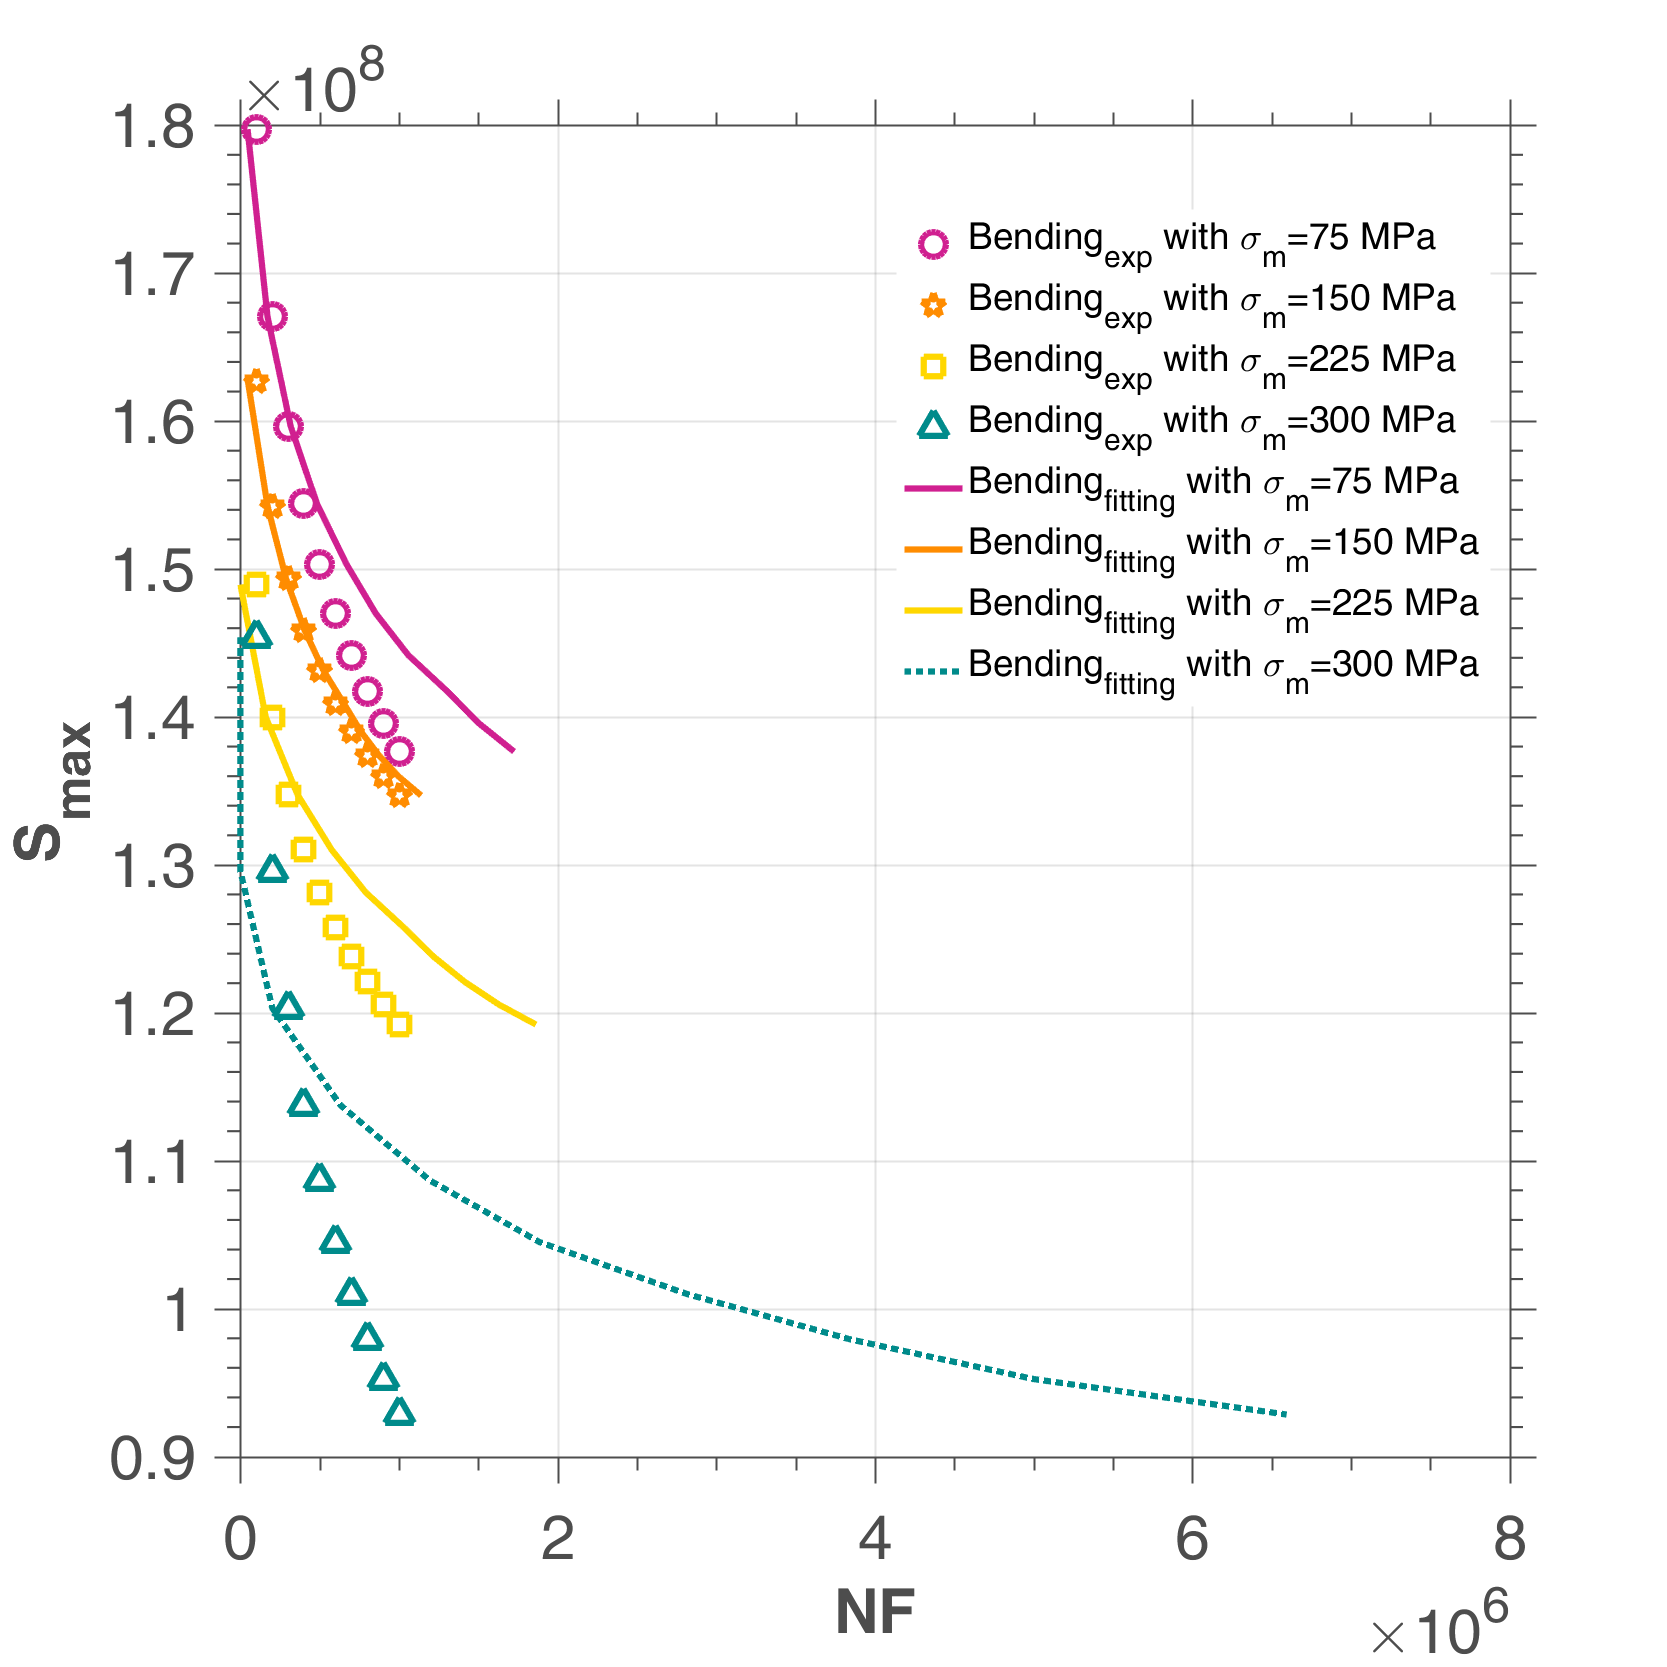
\includegraphics[width=\textwidth]{figures//10HNAP_b1D_m_sn.png} 
	\caption{Wöhler tensile curves for various mean stress values}
	\label{fig.b1Dm10HNAPsn}
\end{figure}


\begin{figure}[!h]
	\centering
	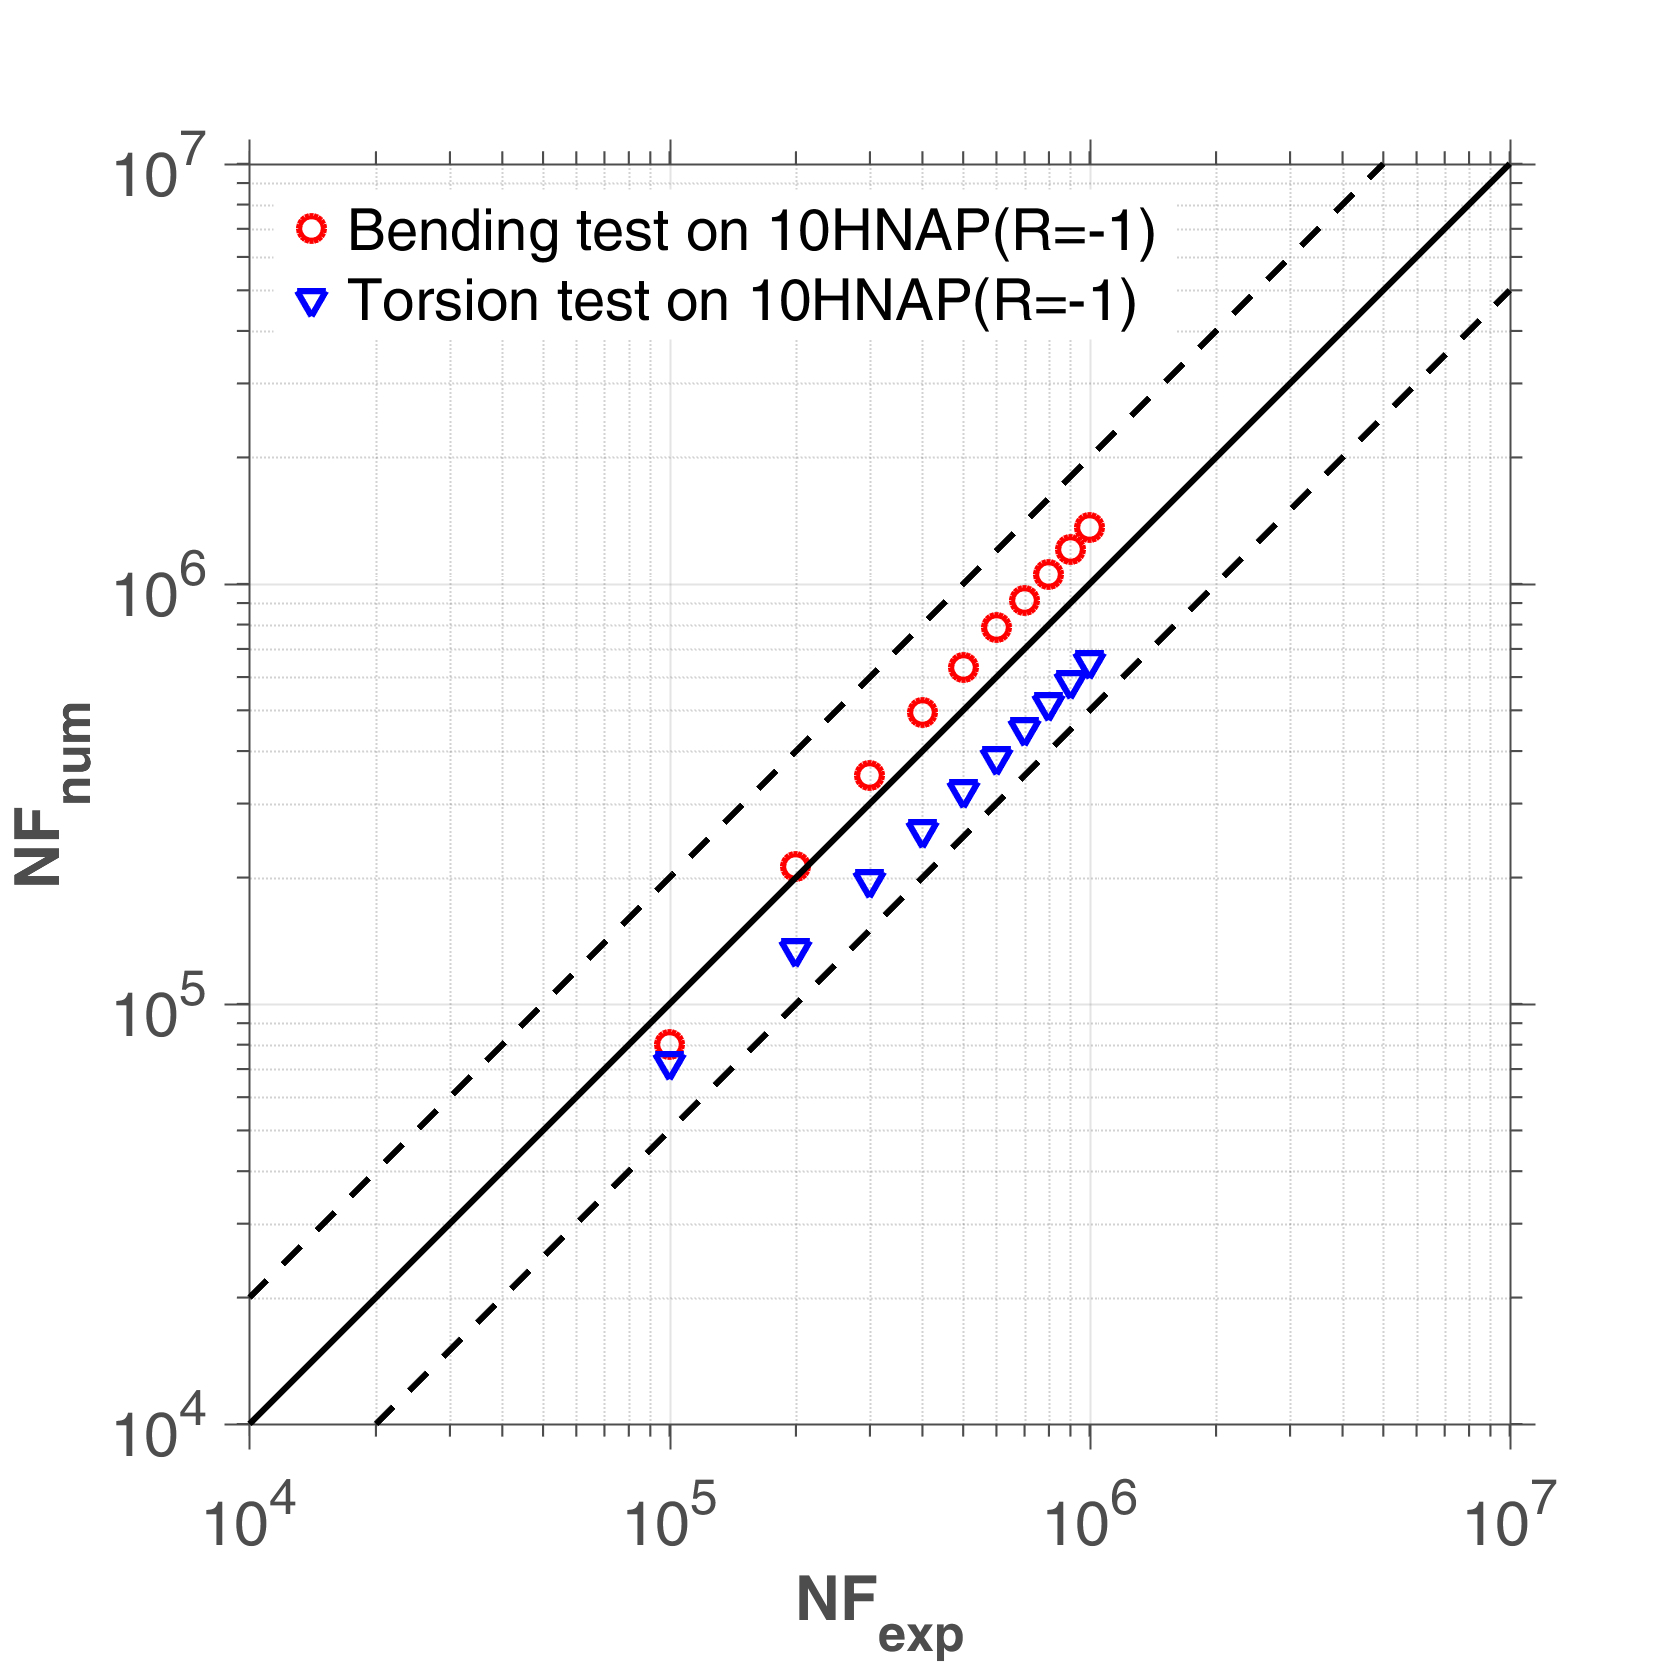
\includegraphics[width=\textwidth]{figures//10HNAP_bt1D_err.png} 
	\caption{Calibration on 10HNAP steel(\cite{jabbado:pastel-00002116}),bending and torsion tests on 10HNAP(R=-1)}
	\label{fig.10HNAP1}
\end{figure}
\begin{figure}[!h]
	\centering
	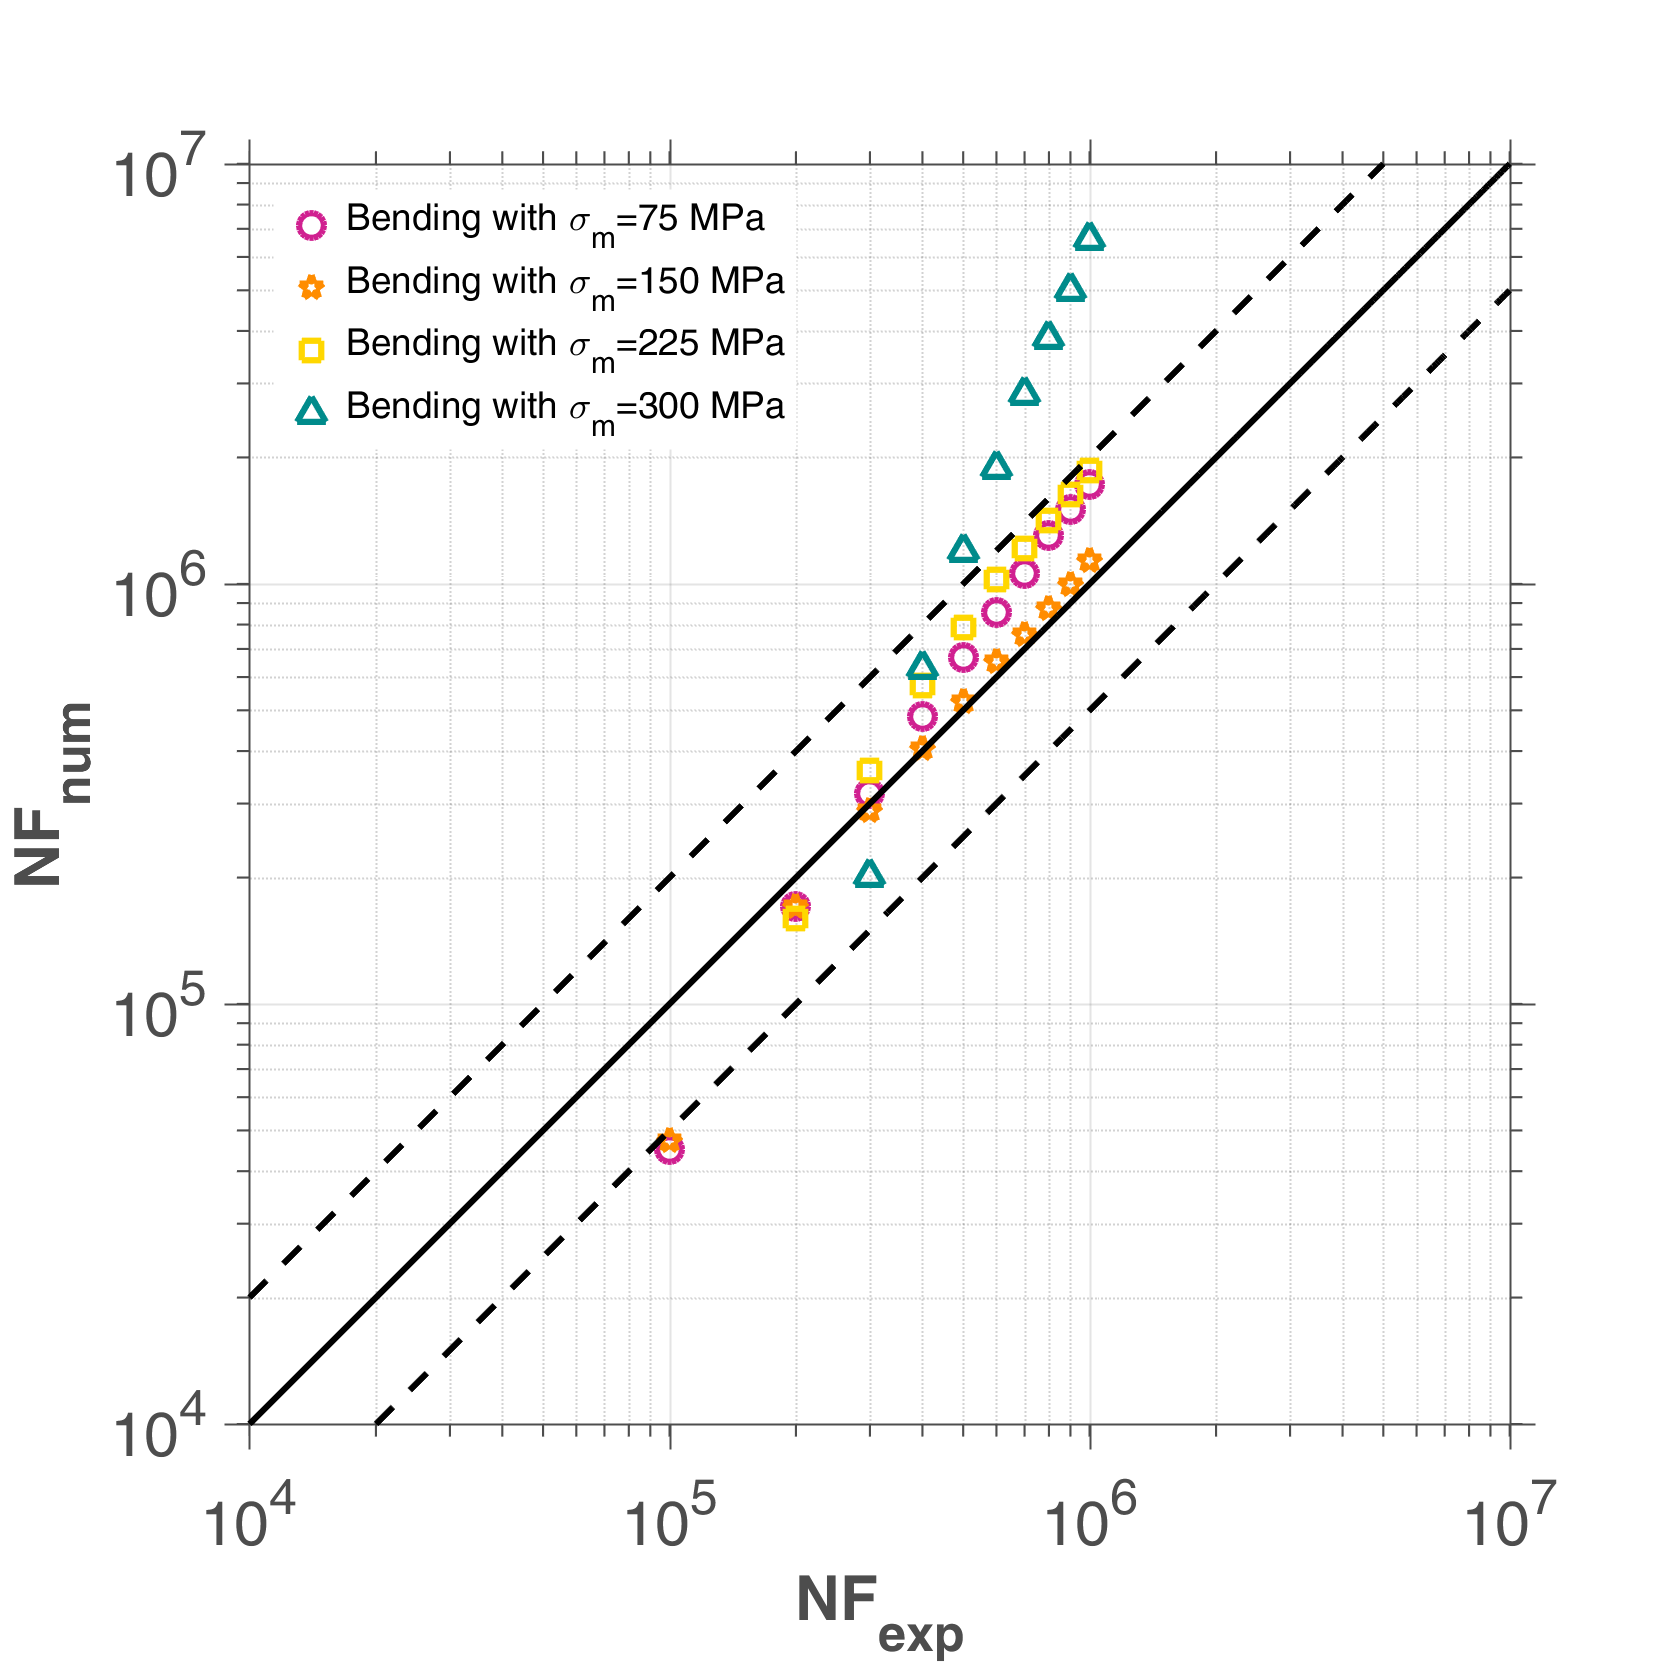
\includegraphics[width=\textwidth]{figures//10HNAP_b1D_m_err.png} 
	\caption{Calibration on 10HNAP steel(\cite{jabbado:pastel-00002116}),bending tests with various mean stress on 10HNAP}
	\label{fig.10HNAP2}
\end{figure}


The prediction results of the tensile tests for various values of the mean stress σm are summarized in \figref{fig.10HNAP2}. These results correlate well with the experimental lifetimes. 

The tests of multiaxial loadings of variable amplitude are plotted in Figures (3.27) and (3.28) as a function of the angle $\alpha_{M}$ and the ratio r. In these figures, the prediction results of the proposed model and that presented by Carpinteri et al. [17]. For the first type of tests ($\alpha_{M} = \pi/8$ and r = 0.2), the best predictions are given by the proposed model.
However, for the second type of tests ($\alpha_{M} = \pi/4$ and r = 0.5), the predictions of Carpenteri et al. [17] are relatively better.

FIG. 3.27(random load results($\alpha_{M} = \pi/8$ and r = 0.2), fail too early due to big $\lambda_+$)

FIG. 3.28(random load results($\alpha_{M} = \pi/4$ and r = 0.4), fail too early due to big $\lambda_+$)

\clearpage
\section{Conclusions}

We work on the stress tensor directly in 3D analysis in stead of using the multidimensional equivalent stress.
The strategy can be made more complex by introducing a local space averaging process in the calculation of the local damage, and by taking more general plastic flows. The energy based fatigue approach takes into account impurities and hardness in the material and is applicable to any type of micro plasticity law and multiaxial load geometry. The time implicit strategy gets rid of cycle counting which is hardly applicable to complex loading, big fluctuation is magnified which reflects the real situation.

There are several advantages and drawbacks of our proposed model. The time implicit method does not take the unit of cycle so as to avoid cycle counting and relevant methods such as rain-flow filter. The possibility to handle different S-N curves corresponding to various materials and load conditions via changing the parameters. We also have the random loading suitability with nonlinear damage accumulation. The drawback is this strategy requires a scale by scale analysis which can be complicated for very high cycle fatigue. However, as introduced above, we can use the optimal time step method to calculate precisely the representative loading history sequence and use scalar integration for the rest of fatigue life. In this way the numerical cost can be dramatically reduced without losing the precision.

Since our method is based on the Dang Van paradigm, to deal with mean stress effect and multiaxial loads we only have the parameter $\gamma$, which is insufficient to fit the experiments.

Also, we need more experimental data and comparison with other peoples' methods.









